% 文件名:Mainbody.tex
% 文件描述:以 scuthesis 四川大学学位论文文档类为基础的 LaTeX 模版
% 作者:LegendaryLeo
% 修改日期:2016年6月3日

% 选用scuthesis文档类,参数master为硕士论文,可选doctor和bachelor,分别对应博士和学士
\documentclass[bachelor,UTF8,hyperref]{./Template/scuthesis}
%\newcommand{\supercite}[1]{\textsuperscript{\cite{#1}}}
\begin{document}
% 设置文档信息
\title{移动端共享图书系统的设计与开发}
\ENGtitle{The Design and Development of Mobile End Sharing Book System}
\CoverTitle{移动端共享图书系统的设计与开发} %封面标题
\author{李博}
\ENGauthor{Li Bo}
\accomplishdate{2019年5月}
\school{计算机学院}
\supervisor{章毅\quad教授}
\ENGsupervisor{Prof. ZhangYi}
\major{计算机科学与技术}
\ENGmajor{Computer science and technology}
\direction{计算机科学与技术}
\ENGdirection{Computer science and technology}
\defensedate{}
\keywords{共享图书,安卓, Restful}
\ENGkeywords{Sharing Book, Android, Restful}
% 设置论文正文前的页码、页眉等
\frontmatter\pagenumbering{Roman}\pagestyle{fancy}\makechaptertitlecenter
% 自动制作标题
\maketitle
% 包含摘要
%!TEX root = ../Manual.tex
\begin{CHSabstract}
	作者本人是一名四川大学的学生,在学习科研活动中经常需要进行学术写作。在使用传统的字处理软件(如~\emph{Microsoft\textsuperscript{\textregistered} Word}~)时,由于其对数学等特殊需求的支持不够友好,因此往往会遇到各种各样的问题,无法高效地写作。作者偶然接触到了~\LaTeX~排版系统,其强大的功能、优美的数学排版和便利的自动化工具等众多优点使人印象深刻,特别适合理工科学生学习和使用。经过了解,发现国际期刊论文主要使用~\LaTeX~进行排版,且国内外许多高校均提供~\LaTeX~的学位论文模版,而我校在这方面的发展还略显不足。在这样的动机驱使下,作者在利用自己较为初级的~\LaTeX~知识,参考了北京大学~Casper Ti. Vector~同学的~\emph{pkuthss}~模版和其他相关文献的基础上,开发了~\emph{scuthesis}~这个适用于四川大学研究生使用的~\LaTeX~学位论文模版。希望此模版能够给各位同学提供一个额外的选择,模版中若有瑕疵,还请各位同学批评指正,留言、新建一个~\emph{ISSUSE}~或~\emph{FORK}~一个新分支修改。


	本文主要对~\emph{scuthesis}~文档模版的使用、功能和实现和进行了简要介绍和说明,并以自身为例进行演示。本模版在~GitHub~的链接为~\url{https://github.com/cuiao/SCU_ThesisDissertation_LaTeXTemplate}.
\end{CHSabstract}

\begin{ENGabstract}
	As a postgraduate of Sichuan University, the author of this document often needs to write academical materials in daily study and research. However, traditional word processing softwares (e.g. \emph{Microsoft\textsuperscript{\textregistered} Word} et. al.) could not provide efficient writing experience due to their lackness support for mathematics et. al. Fortunately, I accessed this \LaTeX~ system by chance and its powerful funtions, beautiful mathematic typesetting effect, the convenient automated kits et. al., which have made a great impress to me, are extremely suitable for science and engineering students. By surveying, international academic jorunals and articles mainly employing this system to typessetting. Additional, many collages and universities from both domestic and overseas are more \LaTeX-friendly by providing their offical dissertation templates in \LaTeX~ comparing with Sichuan University. Motivated by these reasons, based on my kindergarten \LaTeX~ techniques and refering to the \emph{pkuthss} and other documents, I composed this \emph{scuthesis} \LaTeX~ dissertation template for postgraduates of Sichuan University. I hope this template could provide an alternative option for your writing. If there was any flaw in this template, please leave a message to me, creat an new \emph{ISSUSE} in the repo. or \emph{FORK} a new branch to modify.


	This self-contained document is focus on a brief introduction to the using and realization of this template. The link of this template on GitHub is \url{https://github.com/cuiao/SCU_ThesisDissertation_LaTeXTemplate}.
\end{ENGabstract}

% 包含缩略词表
% %!TEX root = ../Manual.tex
\chapter{常用缩略词表}
\emph{例:}\par
\begin{table}[ht]
	\centering
	\begin{tabular*}{\textwidth}{p{0.3\textwidth}p{0.7\textwidth}}
		TUG & \TeX~ Users Group       \\
		bib & Bibliography            \\
		bst & Bibliography Style      \\
		def & Define                  \\
		toc & Table of Contents       \\
		eps & Encapsulated PostScript \\
		cls & Class                   \\
		SCU & Sichuan University
	\end{tabular*}
\end{table}

% 包含符号表
% %!TEX root = ../MainBody.tex

% 常用符号表
\chapter{常用符号表}
\begin{center}
	\begin{tabular}{p{7em}p{20em}}
		$Symbol_{1}$ & 符号$1$ \\
		$Symbol_{2}$ & 符号$2$ \\
		$Symbol_{3}$ & 符号$3$ \\
	\end{tabular}
\end{center}

% 自动制作目录
\maketoc
% 设置论文正文部分的页码、页眉等
\mainmatter\pagenumbering{arabic}\pagestyle{fancy}\makechaptertitleleft
% 包含第一章、第二章等等
%!TEX root = ../MainBody.tex

% 第一章
\chapter{绪论}
本章简单介绍了共享经济的发展背景,我国图书销售和流通情况,以及关于共享图书的国内外研究现状。

\section{项目背景与意义}
    如今,4G 技术已经非常成熟并且普及,5G\cite{Wiki5G} 技术将在未来两年内逐渐普及。移动通信基础设施的完善,
    为移动互联网的发展奠定了坚实的基础。共享经济就是在移动互联网非常发达的基础上发展起来的。
    共享单车,共享汽车,共享充电宝,共享雨伞等一系列共享经济在全球发展火热。

    共享经济主要来源于制度经济学的两大理论:交易成本理论和产权理论\cite{share2018}。 共享经济本质是提高稀缺资源, 
    闲置资源的利用率\cite{SharingEconomy},在资源的生命周期内充分使用资源的价值。共享经济有多种商业模式,
    但共同的特征是其商业的重点是使用权而不是所有权\cite{theory}。共享性需求的产生和发展是经济增长和社会发展的必然结果\cite{think}。共享经济借助网络等第三方平台,将供给方的闲置资源使用权暂时性转移,
    实现生产要素的社会化,通过提高存量资产的使用效率为需求方创造价值,促进社会经济的可持续发展\cite{reason}。实质是使交易成本最小化\cite{trade}。
    可见,共享经济作为一种崭新的经济模式有着无限的潜力。可以举一反三,横向扩展到其他领域,
    比如说共享图书。

    据统计\cite{BookSales},2018 年中国图书销售规模达 894 亿。这表明虽然电子阅读虽然规模不断增长,但纸质图书仍然有很大规模。纸质书
    一个问题是它的利用率并不高,除了学辅教材,专业书等,其他的书籍,我们很少会阅读第二遍。如果这些书籍能够在人与人之间
    相互流通,那不仅提高了图书的利用率,而且有助于保护环境,降低国民的阅读门槛,提升国民的阅读率。
    本文将尝试设计并实现一个共享图书系统,提供一个用户之间共享二手书的平台。通过该平台,将图书真正的在读者之间流动起来。

\section{国内外研究现状}

    2010年,随着 Uber, Airbnb 等共享平台的出现,共享经济作为一种新的经济模式开始发展起来\cite{Airbnb}。国内共享单车共
    享汽车发展的最为火热,然而共享图书却并没有那样流行。根据调查,国内共享图书平台借书人、摩布图书、Book++、
    约书、亿屏借书等发展前景并不乐观,普遍未实现盈利,有的甚至服务已经无法访问。借书人以微信小程序的形式,用户使
    用小程序发布借阅图书,并支付服务费和押金,目前尚未实现盈利。摩布图书\cite{mobu}则是以在广州,成都等地投放共享书柜的形式,
    以租金和会员费,主要以儿童图书为主。至于其它三家服务或网站发现已经无法访问。闲鱼\cite{2taobao}是一个二手物品交易平台,
    它上面的二手书交易量非常可观,但它并不是一个专一面向二手书的交易平台。

\section{研究内容}

本文主要研究设计和开发一套移动端共享图书系统,包括后台和 Android 移动客户端设计开发等工作内容。
 Android 移动端的开发,包括 UI 的设计开发,基本功能的开发实现等,主要实现以下内容:实现基本用户
的注册登录功能;实现基本图书的发布功能,使用户仅仅扫描图书条形码或者手动输入条形码,就能够获
取到所有的图书相关信息,再补充一些发布信息就能够完成图书的发布;实现用户之间的沟通交流。通过该平台,直接在移动端完成
图书的租赁,购买,下单,支付,确认收货,沟通交流等功能。使得用户能够以较低门槛即可共享和租赁图书。
共享图书后台开发的主要内容包括数据实体设计,Restful 服务接口设计,用户的身份认证,根据网
络API获取图书信息等内容。

\section{特色}

\begin{itemize}
    \item 一个类似于 P2P 的用户与用户之间的二手书交易平台。交易过程中完全无第三方的参与。
    \item 移动端的二手书交易平台,用户随时随地都可以互联交易二手书。
    \item 使用简单,低门槛。通过扫描图书条形码即可简单地上传二手书。
    \item 图书交付方式自由,用户之间通过沟通交流,自由决定交付时间地点。
\end{itemize}


\section{论文组织结构}

\begin{itemize}
    \item 第一章,绪论。概括了项目研究背景和目前国内外的研究现状。
    \item 第二章,相关技术。介绍了本项目设计的相关技术的简介。
    \item 第三章,需求分析。分析了共享图书系统的功能需求。
    \item 第四章,总体设计。详细描述了本项目的服务端接口设计,数据库设计,客户端设计。
    \item 第五章,系统实现。详细介绍了服务端的用户登录认证实现和 Android 客户端实现。
\end{itemize}

%!TEX root = ../MainBody.tex

% 第二章
\chapter{相关技术}% 使用\cite{}命令引用数据库中文献
本章介绍在该项目开发中使用到的主要技术。包括 Android, Spring Boot, Spring JPA, Spring Security + JWT, 
Restful, Json, Mysql , 并使用 Maven 和 Gradle 作为依赖管理工具。

\section{Android系统}
Android\cite{Android},是基于 Linux 内核的由 Google 领导和开发的移动设备操作系统,主要为触摸移动设备例如智能
手机和平板设计的。除此之外,还广泛应用在智能电视,智能手表,无线路由,智能冰箱,智能汽车等设备
上。Android 主要运行在 ARM 处理器架构的设备上,也有少量 X86 架构的 Android 设备。

目前 Android 的市场占有率高达 85.9\%。2008 年 9 月 23 日,第一步 Android 手机 HTC Dream 发布。从最初的 Android 1.0,1.1,
 1.5 逐渐到2.0,3.0, 到目前最新的 Android Pie 9.0,API 级别为 28,在 10 年时间内,Android 经过了十余
 次的迭代更新。核心的 Android 源代码以 Android 开源项目(AOSP)而著名。2017年,Android设备超越 Microsoft Windows,成为全球第一大操作系统。

\begin{itemize}
    \item Android Activity 组件
    
    Activity\cite{Activity} 相似于网页的一个页面,不过它是安卓操作系统上独有的页面。它是通过 xml 的方式描述
    安卓的页面布局。由于移动设备的独特性,所以 Android 系统的屏幕一次只显示一个 Activity,不过在 Activity 内
    可以包含多个 Fragment 片段。Fragment 类似于 Activity,但它不能单独显示在 Android 设备页面,而是只能包含
    在 Activity 内,同样有 xml 文件定义的布局。

\end{itemize}



 \section{Spring框架}
Spring,即 Spring Framework\cite{SpringFramework},是 Java 平台的控制反转容器的应用框架。它是一个开源项目,作为 Enterprise
JavaBean 模型的替代方案。在诞生之初,Spring 的主要目的是用来替代更加重量级的企业级 Java 技术\cite{SpringInAction},
Spring 为企业级 Java 开发提供了一种相对简单的方法,通过依赖注入和面向切面编程,用简单的 Java 对象
实现 EJB 的功能。

Spring 框架包含了一些模块用于提供服务\cite{WikiSpring} 包括 Spring 核心容器,面向切面编程,认证和授权,数据访问,控制反转容器,消息,模型-视图-控制器,事务管理等。
% \begin{itemize}
%     \item   Spring核心容器: 这是Spring的基础模块,提供spring 容器(BeanFactory 和 ApplicationContext)。
%     \item   面向切面编程:允许实现横切的特点。
%     \item   认证和授权:配置安全过程,通过 Spring Security子项目支持很多标准,协议和工具。
%     \item   数据访问:使用java平台的JDBC,关系数据库管理系统,对象关系映射工具,与非关系型数据库。
%     \item   控制反转容器: 配置应用组件和Java对象的生活周期管理,主要通过依赖注入完成。
%     \item   消息:通过Java消息服务(JMS)的方式配置注册消息队列的消息侦听器,通过标准的JMS API 提升发送消息。
%     \item   模型-视图-控制器:基于 HTTP 和 servlet 的框架提供面向 web 应用和 RESTful Web 服务的自定义和扩展。
%     \item   远程访问框架:可配置的远程程序调用风格的通过网络支持 Java 远程方法调用的Java对象传输。和包括 Web 服务的
% 基于HTTP的协议。
%     \item   事务管理:统一了事务管理API与Java对象的协作事务。
% \end{itemize}

\section{Spring Boot框架}
虽然 Spring 的组件代码是轻量级的,但它的配置却是重量级的 \cite{SpringBootInAction} 。
 Spring Boot \cite{SpringBoot} 将很多魔法带入 Spring 应用程序的开发之中,包括下面四个核心方面:

\begin{itemize}
    \item    自动配置:针对很多 Spring 应用程序常见的应用功能,Spring Boot 能提供相关配置。
    \item    起步依赖:告诉 Spring Boot 需要什么功能,它就能引入需要的库。
    \item    命令行界面:这是 Spring Boot 的可选特性,借此你需要代码就能完成完整的应用程序,无需传统项目构建。   
    \item    Actuator: 让你能够深入运行中的 Spring Boot 应用程序,一探究竟\cite{SpringBootInAction}。
\end{itemize}

\section{Spring Data JPA技术}
JPA 是 Java Persistence API 的简称。是 Spring 集成的数据持久化框架。目前市场上的 ORM(object/relational metadata)框架由 Mybatis,
Hibernate,Spring Data JPA\cite{SpringDataJPA2}. Spring Data JPA 是一种使用相对简单的方式。

JPA 包含三方面的内容:API 标准,面向对象的查询语言,ORM 元数据的映射。JPA 的宗旨是为 POJO 提供持久化标准
规范\cite{SpringDataJPA}。

Spring Data JPA 大大简化了我们 DAO(Data access object)层的开发,使我们只要创建普通的 Java 对象,
即pojo,再加上标记,就可以通过 JPA 的 API 操作数据库。

\section{Spring Security安全框架}
Spring Security\cite{SpringSecurity} 是一个强大的高度可定制的认证和入口控制框架。它是事实上的保护基于 Spring 的应用的标准。
Spring Security 是专注于 Java 应用的认证和授权框架。Spring Security 最初在2003年后半年开始于 Acegi Security, 
由 Ben Alex 开发,2004年在 Apache 证书下发布。接下来,变成了官方的 Spring 的一个子项目。

Spring Security的特点:

\begin{itemize}
    \item 对于认证和授权来说都是易于理解和可扩展的。
    \item 保护应用免受会话攻击,点击劫持,扩展请求伪造等攻击。
    \item 继承了 Servlet API。
    \item 可选的与 Spring Web MVC 集成。
\end{itemize}

\section{Maven构建工具}
Maven 是 Apache 基金会下的一个项目,即 Apache Maven。官方定义\cite{Maven}: Apache Maven 
是一个软件项目管理和理解工具。基于项目对象模型(POM)的概念,Maven 可以从一个中心消息
片管理一个项目的构建,报告和文档。维基百科定义\cite{WikiMaven}:
 Maven是一个主要用于 Java 项目的自动工具。

% Maven定位构建软件的两个方面:第一,它描述如何构建软件,第二,它描述依赖。不像早期的Apache Ant,它使用惯例构建软件,
% 只有异常需要写下来。一个XML文件描述项目如何构建,它对外部模块和组件的依赖,构建顺序,目录,需要的插件。它天生就是来处理
% 定义好的目标,执行特定的定义好的任务例如编译代码和打包。

Maven 从一个或者多个仓库例如 Maven 2 中心仓库动态地下载 Java 库和 Maven 插件并存储到本地缓存中。 本地下载地库可以被本地项目更新,
公共仓库同样可以更新。Maven 同样可以用来构建和管理其他语言的项目例如 C\#,Ruby,Scala,或者其他语言。

\section{Gradle构建工具}
Gradle\cite{Gradle} 是一个开源自动构建系统,在 Apache Ant 和 Apache Maven 的
概念之上,引入了基于 Groovy 的域定义语言(DSL)来替代 Maven 使用的用来声明项目配置的 XML 形式。
Gradle 使用有向无环图("DAG")来决定任务的执行顺序,Gradle 也会缓存任务的输出,当 Gradle 发现任务的输入输出在构建运行时改变,这个任务将会再次执行。

% Gradle使用有向无环图("DAG")来决定任务的执行顺序。Gradle 被设计为多项目构建的。它支持通过智能的决定构建树的
% 哪部分过期增量构建;任何任务独立的部分不需要再次执行。Gradle 检查构建的输入输出来查看自上次构建调用后一个任务的输出是否
% 改变,如果没有,这个任务被认为是最新的,将不会被执行。Gradle 也会将任务配置作为输入的一部分。Gradle 允许并行的任务执行和通过一个 Worker API来进行内部任务,并行化
% 导致了更快的性能。Gradle 也会并行下载依赖元数据。

% Gradle 也会缓存任务的输出。如果一个任务已经在另一台计算机执行过,Gradle 会跳过本地执行,从构建缓存中获取任务输出。
% 这种典型的用例让CI构建推送到一个共享的任务缓冲区,并且允许开发者拉取它。本地构建缓存同样能够被使用来重用以前在相同计算机
% 上构建的输出。

% 当Gradle发现任务的输入输出在构建运行时改变,这个任务将会再次执行。这个任务将使用增量的API来知道具体哪些文件发生了改变。
% 有了这个消息后,这个任务不需要重新构建所有。

\section{Mysql数据库}
MYSQL\cite{WikiMysql}是一个开源关系型数据库管理系统。

Mysql 是常用的开源数据库,被很多著名的网站使用,包括 Google,Facebook,Twitter,
Flickr,YouTube。Mysql 是用 C 和 C++ 写的, 支持很多平台,包括 Windows,MacOS,Unix,以及 Linux 的多个
发行版,你甚至可以自行下载它的代码来编译。它支持存储百万级的数据存储。不仅如此,Mysql 还参考了 SQL 标准,并对 SQL 
提供了很好的支持。它被设计由独立模块组成的多层服务器设计,被设计为完全多现成的,并且提供了事务和非事务的存储
引擎供你选择。它在 MyISAM 存储引擎中使用非常快的 B 树索引。Mysql 支持大的数据库,官方曾经使用 MySQL 服务器
包含了 5000 万条记录。为多种编程语言提供了 API 接口\cite{MysqlMainFeature}。

Mysql 被设计为 Server 和 存储引擎分离的,并且存储引擎是可插拔的,你可以从 MySQL 服务器中载入和卸载存储引擎。
不同存储引擎提供了一些不同的特点,默认的存储引擎是 InnoDB。Mysql 支持的存储引擎有 InnoDB,MyISAM,Memory,
CSV,Archive,Blackhole,NDB,Merge,Federated,Example 等。这些引擎之间的不同在于提供了不同的特点,让你根据
你的数据特点选择。主要不同在以下方面: B 树索引的支持,备份点实时恢复的支持,簇数据库的支持,簇索引,是否压缩数据,
是否缓存数据,是否加密数据,是否支持外键,是否支持全文索引,是否支持地理空间数据类型,是否支持地理空间索引,是否支持哈希
索引,是否支持缓存索引,支持的锁粒度,MVCC 的支持,赋值的支持,存储容量限制,T 树索引的支持,事务的支持,数据字典的更新等\cite{MysqlNewFeature}。

\section{Restful原则}
REST ( Representational State Transfer),表达性状态传输, 是一种创建规模网络服务的软件架构方法。
术语 REST 由 Roy Field 在他的博士论文中提出,解决了很多原则问题。包括了
以下原则\cite{RESTfulService}:

\begin{itemize}

\item Uniform interface

REST 的核心是资源,资源由统一资源定位符(Uniform Resource Identifiers , URIs)标识,资源与它们的
表示(它们提供给客户端的格式)分离。REST 没有具体要求格式,但通常包括 XML 和 JSON。

除此之外,资源表述是自我描述性的,更具体地说,这意味着成功的回复处理必须返回足够充分的信息。

REST 的另一个不同的属性是客户端完全是通过超媒体交互的,由应用服务器动态提供,除了端点,客户端对如何与 RESTful
服务交互一无所知。这种约束被称为应用状态引擎超媒体 ( Hypermedia as the Engine of Application State , HATEOAS )\cite{RESTfulService}。

\item Client-Server模型

客户端服务器模型表示 REST 接受客户端关注点的分离,例如用户交互或者用户状态管理,与服务器关心的
存储和规模性。

这种解耦确保,提供一个达成一致的接口,客户端和服务器能够独立的开发。它同样减少了复杂性,提升了性能调整
的效率。

\item 无状态

REST提倡无状态。服务器不保存客户端的状态。所有需要执行操作的请求信息都包含在请求中(作为URL,请求
体,HTTP头部的一部分)。

\item 可缓存的

RESTful web服务必须提供缓存能力。服务器能够暗示如何和缓存回复多久。客户端可以使用缓存的回复而不是联系服务器。

\item 层级系统

这种客户端和服务器的沟通风格,客户端并不清楚它们正与哪台具体的服务器交互。这种属性允许引入中间
服务器,例如处理安全或者提供负载均衡能力的服务器。

\item 按需代码

即使是REST架构的一部分,这个原则也是可选的。服务器可以临时的扩展客户端的功能通过传输可执行的代码。
例如可以传输给基于web的客户端 JavaScript 代码来自定义功能。

\end{itemize}
\section{JSON数据格式}
JSON, JavaScript Object Notation\cite{WikiJSON}. JavaScript 对象符号,是一种人类易读的文本 , 用来传输数据对象
包含属性-值键值对和数组数据类型的文件格式。它是一种非常常见的以部的浏览器-客户端沟通的数据格式。

JSON是语言独立的书写格式,衍生自 JavaScript。官方的 Internet 媒体类型是
application/Json。JSON 文件名使用后缀.json。

\section{JWT身份认证}
JWT(JSON Web Token)\cite{JWT}是一个开源标准(\href{https://tools.ietf.org/html/rfc7519}{RFC 7519}),定义了
在团体之间使用JSON对象安全传输信息的切确和自我包含方式。这条信息可以被验证,因为它是数字签名的。JWT 可以使用
密匙签名(使用HMAC算法)或者公共/私有密匙对使用 RSA 或者 ECDSA。

JWT 被用来授权是最常见的使用场景。一旦用户登录,每个后续请求都包含 JWT,允许用户获取路由,服务,和 token 许可的资源。
如今使用 JWT 的单点登录特点被广泛使用,因为它的小的负载头部和在不同域间轻松使用的能力。





%!TEX root = ../MainBody.tex

%第三章
\chapter{需求分析}
共享经济的发展如火如荼 \cite{SharingEconomy2},图书平均保有量也在稳中增长,在共享图书系统开发之前,需要具体分析用户需求,确保
符合并满足用户的需求。

\section{可行性分析}
在项目开发和需求分析之前,需要系统地分析项目开发和未来交付运行地可行性。

\begin{itemize}
	\item 市场可行性
	
	据统计分析\cite{BookMarketReport2018},2018 年中国全国图书零售市场规模维持两位数增长,2018 年
	中国图书零售市场码洋规模达894亿,同比上升 11.3\%,增速相比 2017 年有所放缓,但依然维持两位数
	增长。新书品种维持平稳,新书定价持续上升。2018 年新书平均单册码洋 41.5 元。
	
	中国图书这么庞大并且持续增长的销售规模,表明人们对于纸质书籍依然有很大的需求,而且表明
	个人手头都有一些已经购买阅读过的闲置书籍。随着纸价的上涨,图书的平均单价也在上涨,这
	也给个人获取书籍增加了不少的成本。如果能够让这些图书在消费者之间流通起来,将大大减少人们的阅读
	成本,从而使人们在相同的成本下能够阅读到更多的书籍,也提高了书籍的利用率,减少了对纸的需求,
	间接保护了生态环境。
	
	本平台将提供消费者之间图书流通的平台,让书籍在人们之间流通起来,看起来是完全可行的。

	\item 技术可行性
	
	目前,以spring开发框架进行后端开发非常流行,而且技术比较成熟,Spring 框架也使得开发 Restful
	形式的服务非常方便。Spring 还集成了 Spring JPA,Spring Security 等子模块,这大大简便了后端
	的开发。Spring 基于 POJO 的开发方式相对与企业级的 Java Bean 也非常轻量级。开发者能够快速掌握 Spring
	后端开发。笔者学习过相关技术,并且曾经使用相关技术做过一个个人博客系统。对相关技术比较了解,所以后端
	开发技术上是可行的。

	前后端分离\cite{backendDispart}的开发方式,思想也比较成熟,并且得到了广泛的应用。前后端的解耦大大加快了项目的开发效率。
	前后端可以约定交互的接口,然后同时进行开发。而且 Spring 只需要简单配置就能够开发 Restful 服务,暴露
	Restful 接口。

	Android 从最初的 Android 1.0,到当前的 Android 9.0 ,API 也非常成熟,资料文档非常齐全。Android 也有
	很多网络库和 Json 库,使得 Android 能够非常容易地访问Restful形式地服务。笔者在寒假之前就开始学习 Android 开发,
	边学习边开发,之前也尝试开发过一些 Demo,所以 Android 端技术上也是可行的。

	所以从技术地角度来讲,是完全可行的一个项目,技术非常成熟,能够迅速进行开发。
	
\end{itemize}



\section{需求概述}
主要的需求是用户的发布图书,并且浏览平台上的闲置图书,并在平台上进行个人
已发布图书基本管理,对他人图书的借阅,归还等。还包括了基础的登录注册功能。总体划分为以下几个功能
模块:

\begin{enumerate}
	\item 首页图书列表,底部包含一个导航,上面显示的是本地缓存的图书列表信息,通过上划,获取更多的图书信息。
	\item 发布图书,点击发布按钮扫描图书条形码或者手动输入图书 ISBN,最终都将图书 ISBN 作为参数,请求服务器,获取服务器返回的图书信息,
	然后用户补充图书信息,例如个人描述,出售租赁价格等,并发布图书。
	\item 最近联系人列表,显示当前用户的最近联系人列表。
	\item 我的首页,显示与我相关的信息选项,包括我的发布,我的钱包,退出登录,清除缓存等。
	\item 我的发布,显示我已经发布的图书列表。
	\item 图书详情,显示图书的详细信息,包括标题,作者,ISBN,描述,出版时间,价格等详细信息。
	\item 我的钱包,显示我的钱包余额。
	\item 注册登录,这是两个不同的界面,一个用来通过邮箱和用户名进行注册,一个用用户名或者邮箱来登录。
	\item 下订单,用户点击图书详情的购买或租赁,进行下单,并转到支付界面。
	\item 支付,用户进行支付。
\end{enumerate}

\section{用户角色}
在该系统中,用户拥有多种角色,包括用户,租书消费者,购书的消费者,书籍拥有者,交付员。当用户注册登录后,便成了该平台的用户。
当用户发布了一本图书,该用户就是一个书籍拥有者,如\cref{owner}。当该书被租出或卖出时,该用户在交付过程中可能成为交付员,如\cref{deliver},负责将图书交付给消费者。
当用户在平台上购买了某本书时该用户是购书消费者,如\cref{costumer}。当用户租了某本书时,用户是租书消费者,如\cref{costumer}。

\begin{figure}[h]
	\centering
	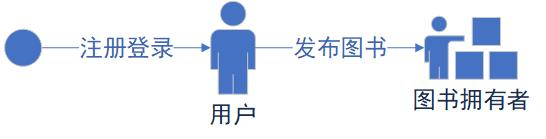
\includegraphics[scale=0.65]{Chapters/UML/owner.jpg}
	\caption{拥有者}
	\label{owner}
\end{figure}

\begin{figure}[h]
	\centering
	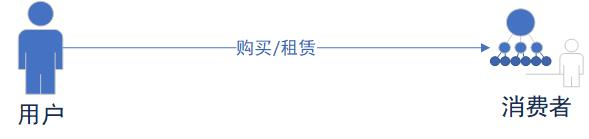
\includegraphics[scale=0.65]{Chapters/UML/costumer.jpg}
	\caption{消费者}
	\label{costumer}
\end{figure}

\begin{figure}[h]
	\centering
	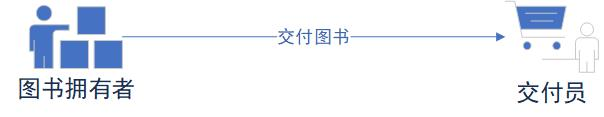
\includegraphics[scale=0.65]{Chapters/UML/deliver.jpg}
	\caption{交付员}
	\label{deliver}
\end{figure}

\section{系统业务流程}
基于 Android 的图书共享系统,需要满足用户基本的登录注册,发布图书,借阅租赁图书,沟通交流的需求。通过手机简单
的扫描图书条形码即可简单的发布图书,在手机上即可浏览图书相关信息,并且通过手机下单进行租赁,购买沟通等
功能。\cref{system_bussness_process}是完整的系统业务流程图。

\begin{enumerate}
	\item 发布图书,用户通过手机客户端扫描或手动输入图书 ISBN,获取到图书信息,进一步补充图书信息,租赁价格,出售价格,
	个人描述,点击发布。
	\item 租赁图书,用户在某本书下通过与主人沟通协商交易信息,就价格和交付方式达成一致后点击租赁,生成订单,进行支付,等待
	交付。租赁期限内,归还图书。订单完成。
	\item 购买图书,在双方协商一致后,下单,支付,交付。订单完成。
	\item 沟通交流,当用于对某本书有兴趣时,可以跟该书主人沟通交流。
\end{enumerate}

\begin{figure}[h]
	\centering
	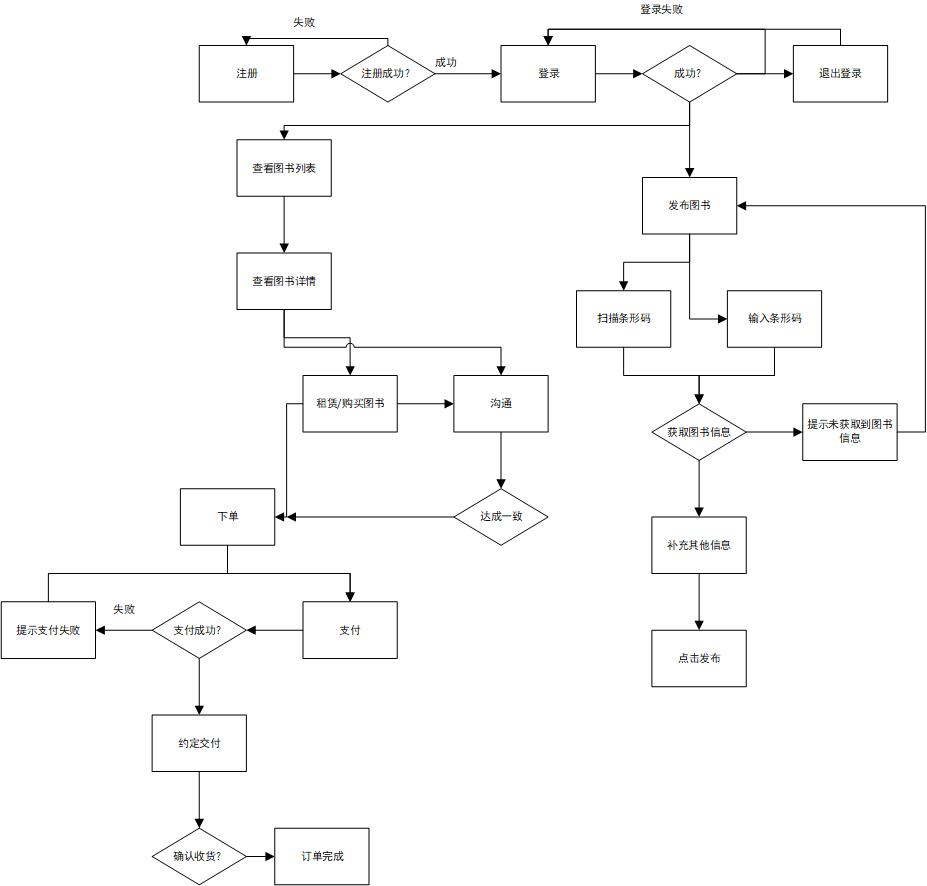
\includegraphics[scale=0.6]{Chapters/UML/system_bussness_process.jpg}
	\caption{系统业务流程图}
	\label{system_bussness_process}
\end{figure}

\section{功能需求}
\cref{function_structure}是功能结构图

\begin{figure}[h]
	\centering
	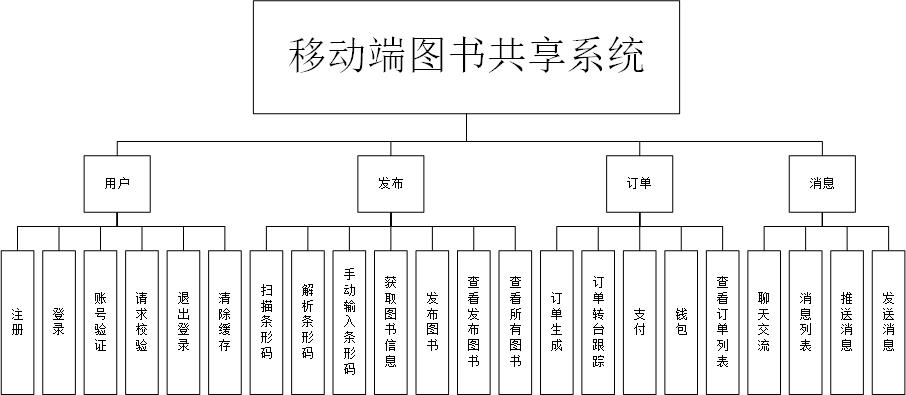
\includegraphics[scale=0.65]{Chapters/UML/function_structure.jpg}
	\caption{功能结构图}
	\label{function_structure}
\end{figure}

\begin{itemize}
	\item 注册, 客户端的用户注册。
	\item 账号验证,用户注册时验证账号是否合法。
	\item 登录,客户端用户登录。
	\item 请求校验,对用户请求的合法性进行角色权限判断。
	\item 扫描条形码,移动端调用详细扫描条形码。
	\item 解析条形码,对扫描到的条形码进行解析。
	\item 手动输入条形码,用户自行输入条形码。
	\item 获取图书信息,根据 ISBN 获取图书相关信息。
	\item 发布图书,客户端完成用户图书的发布。
	\item 订单生成,用户下单,服务器生成相应订单。
	\item 聊天交流,用户之间的沟通协商。
	\item 订单状态跟踪,对订单状态的改变。用户下订单时,订单处于未支付状态。用户支付,订单变为已支付状态。订单交付,订单变为完成状态。
	\item 支付,对订单进行支付,检查用户账户余额,并完成扣款。
	\item 钱包,对用户账户的余额进行操作,增加,扣除。
	\item 查看订单列表,获取用户完整的订单列表。
	\item 查看发布图书,获取用户的所有已发布的图书。
	\item 查看所有图书,获取所有用户发布的所有图书。
	\item 退出登录,完成用户退出操作。
	\item 清除缓存,清除客户端缓存数据。
	\item 消息列表,获取用户的聊天记录。
	\item 推送消息,用户收到来自其他人的消息时,推送消息。
	\item 发送消息,发送给其他用户消息。
\end{itemize}

\section{数据需求}

\begin{itemize}
	\item 用户账户信息,在注册和登录时,用户在客户端完成信息补充。
	\item 图书 ISBN, 通过条形码扫描解析或者用户手动输入获取 ISBN。
	\item 图书详情的 Json 数据,通过客户端获取到的 ISBN,从服务器获取 Json 数据,服务器从 books.googleapis.com 获取关于图书的 Json 数据信息。
	\item 订单数据,用户下单后,服务端应返回完整的订单信息。
	\item 订单列表,从服务器获取单个用户的所有订单信息。
	\item 聊天数据,用户登录后,从服务器获取历史信息。
	\item 钱包数据,查看用户余额。
	\item 用户图书列表,从服务器获取单个用户已发布的图书列表。
	\item 图书列表,从服务器获取所有已发布的图书列表。
\end{itemize}

\section{本章小结}
本章主要完成了共享图书的需求分析,首先对系统开发的可行性进行了分析,从经济可行性、技术可行性两个方面进行
了分析。然后对共享图书的功能需求进行了分析说明。


%!TEX root = ../MainBody.tex

%第四章
\chapter{总体设计}

\section{系统总体结构设计}
\cref{all_module_design}是系统总体结构设计。左边是服务器端,暴露 Restful 服务接口,响应客户端的 HTTP 请求,
返回 Json 数据。右边是 Android 客户端,发起 HTTP 请求,将得到的请求结果保存在本地 Sqlite 数据库中。

\begin{figure}[h]
	\centering
	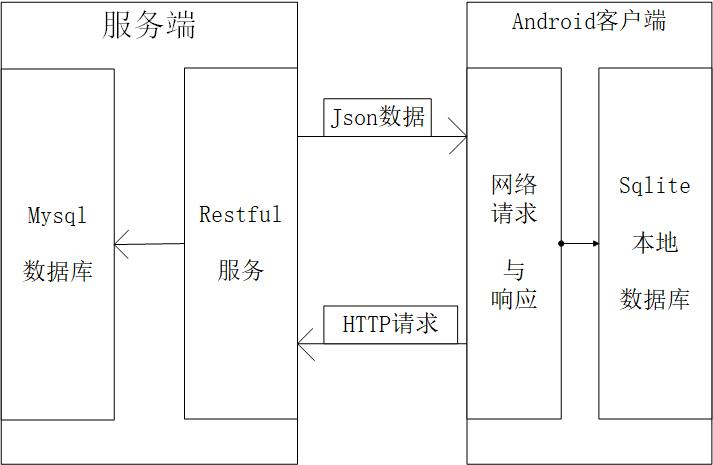
\includegraphics[scale=0.5]{Chapters/UML/system_structrue.jpg}
	\caption{系统总体结构设计}
	\label{all_module_design}
\end{figure}

\begin{figure}[h]
	\centering
	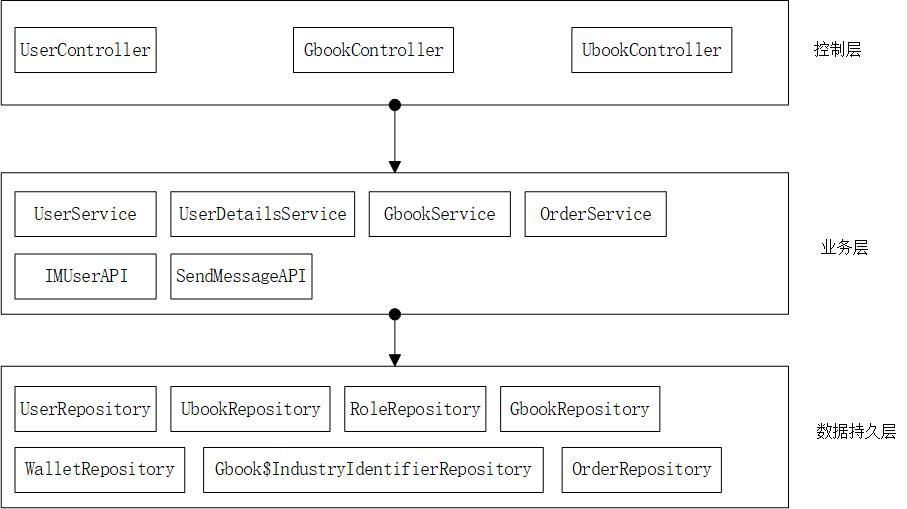
\includegraphics[scale=0.6]{Chapters/UML/system_level_design.jpg}
	\caption{服务端系统分层设计}
	\label{system_level_design}
\end{figure}

\section{服务端系统分层设计}
\cref{system_level_design}是服务端系统分层设计。项目结构分为控制层,业务层和数据持久层。控制层负责响应用户
请求,调用业务层完成请求。业务层进行相关处理,并调用数据持久化层方法完成业务逻辑。数据持久层专一负责数据的存储与
查询等操作。

\section{系统业务流程}

\cref{user_login}是用户登录流程图。用户在客户端输入用户名和密码,将参数上传至应用服务器,服务器首先
判断账户是否存在,然后判断密码是否一致,如果通过判断,则生成 token,并返回给客户端。客户端拿到 token,算作
成功的一次登录。

\begin{figure}[h]
	\centering
	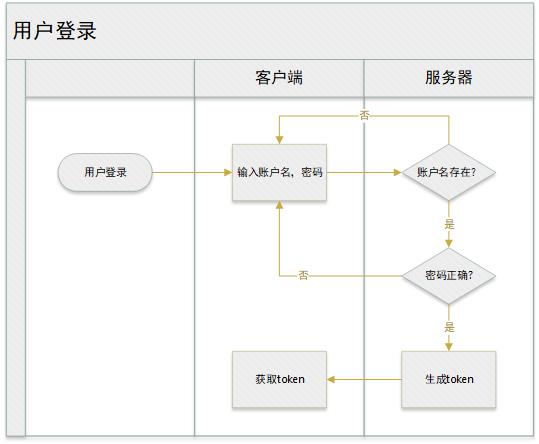
\includegraphics[scale=1]{Chapters/UML/user_login.jpg}
	\caption{用户登录流程图}
	\label{user_login}
\end{figure}

\cref{user_register}是用户注册流程图。用户在客户端输入帐户名,异步发送给应用服务器,服务器判断账户名是否已
存在,如果不可用,则返回错误信息;然后用户输入邮箱,同样异步发送到应用服务器判断是否可用;之后用户在客户端
输入密码和二次密码,两次密码不仅要一致,而且要在客户端判断是否符合密码强度;上述都通过后,请求服务器;服务器
创建账户并返回信息。
	
\begin{figure}[h]
	\centering
	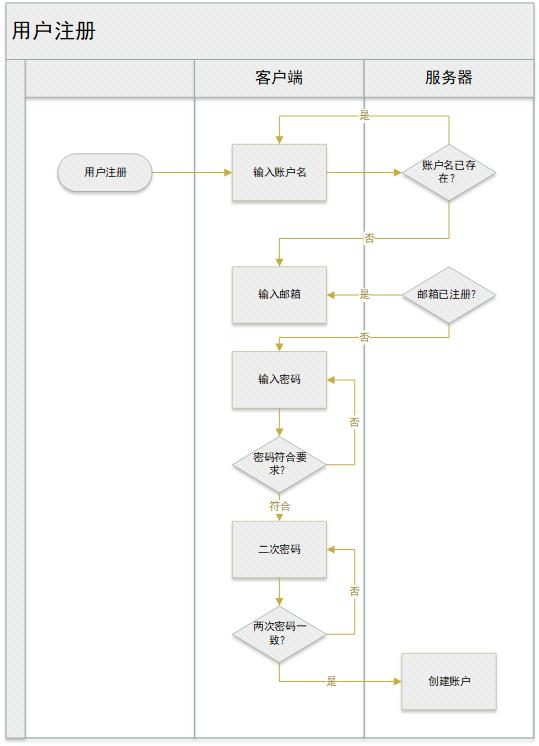
\includegraphics[scale=0.8]{Chapters/UML/user_register.jpg}
	\caption{用户注册流程图}
	\label{user_register}
\end{figure}

\cref{user_release}是用户发布图书流程图。用户在客户端选择扫描条形码或手动输入来获取图书 ISBN,然后
请求应用服务器获取图书相关信息,如果应用服务器没有该书信息,则应用服务器请求三方服务器获取图书信息,成功
获取到后,首先保存在本地应用服务器中,然后返回给客户端相关的图书信息。客户端获取到图书信息后,进一步补充
相关信息,然后再次发送请求到应用服务器,完成发布。

\begin{figure}[h]
	\centering
	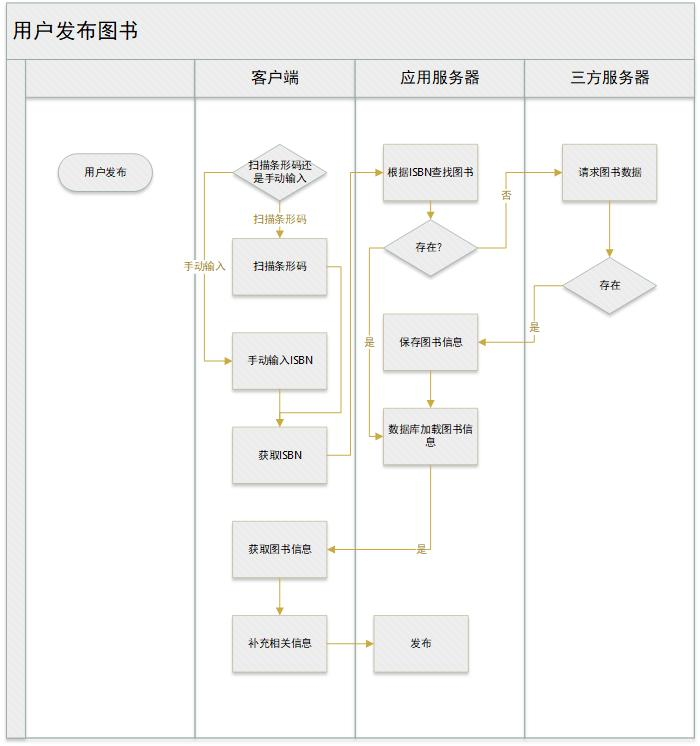
\includegraphics[scale=0.7]{Chapters/UML/user_release.jpg}
	\caption{用户发布流程图}
	\label{user_release}
\end{figure}

\cref{user_rent_or_buy}是用户租赁购买图书流程图。用户在客户端选择租赁或购买,请求应用服务器,服务器生成
响应的订单信息并返回。用户在客户端选择订单进行支付,服务器根据用户账户余额来判断是否能够完成支付。如果支付
完成,则订单进入约定交付状态,用户和图书拥有者通过沟通交付订单。如果是购买,则当用户点击收获后订单完成。否则,
如果是租赁,则订单进入待归还状态,在图书拥有着点击确认归还后,订单完成。

\begin{figure}[p]
	\centering
	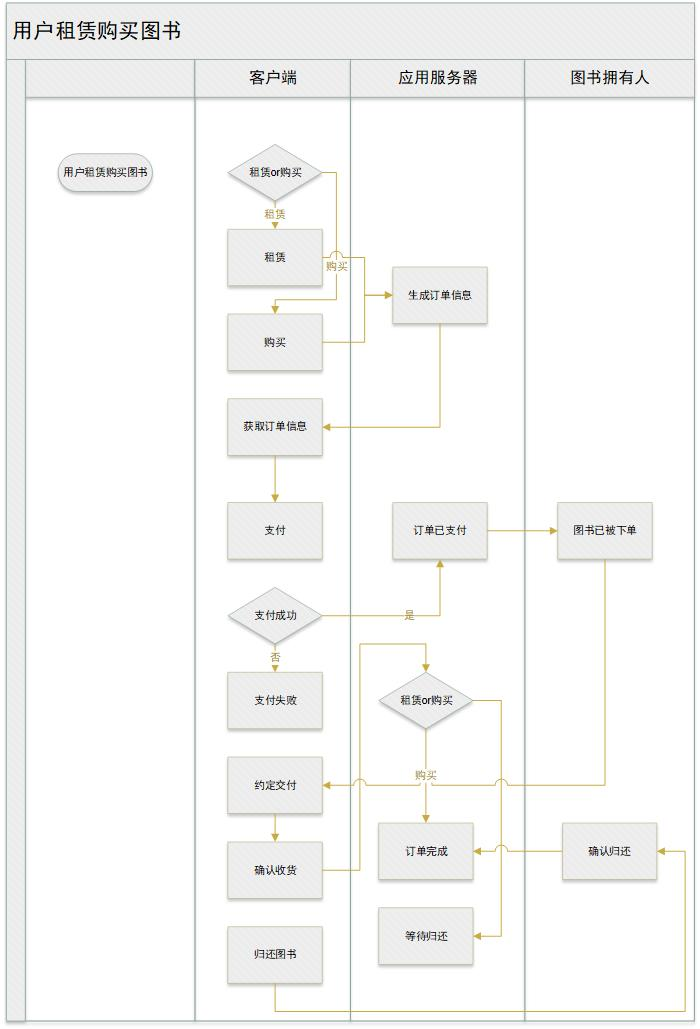
\includegraphics[scale=0.75]{Chapters/UML/user_rent_or_buy.jpg}
	\caption{用户租赁购买图书流程图}
	\label{user_rent_or_buy}
\end{figure}

\section{ Android 客户端界面与功能设计}
\cref{android_ui}是 Android 客户端功能设计。

未登录用户可以通过首页查看图书列表,和图书详情信息,但是不能发布图书。

登录用户拥有未登录用户的所有功能,并且可以发布图书,以购买或租赁图书的方式下单并进行支付。

根据设计和需求分析,将客户端划分为以上用户界面,下面对各个界面进行介绍:

\subsection{首页}

\begin{figure}[h]
	\centering
	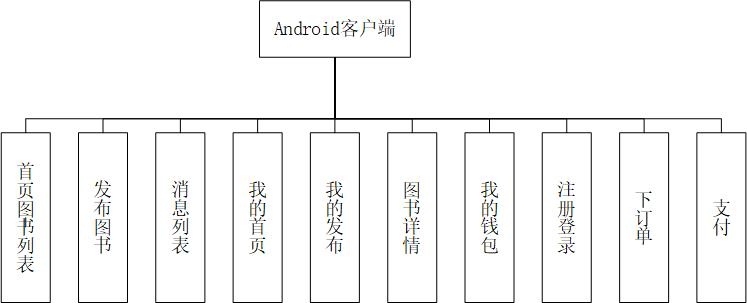
\includegraphics[scale=0.7]{Chapters/UML/android_ui.jpg}
	\caption{移动端界面功能设计}
	\label{android_ui}
\end{figure}

\cref{main_ui}是 Android 的客户端主页,包含图书列表和最下方的导航栏。用户通过下滑操作查看图书列表,通过点击某项,
	查看图书具体信息。
	
	\begin{figure}[h]
		\centering
		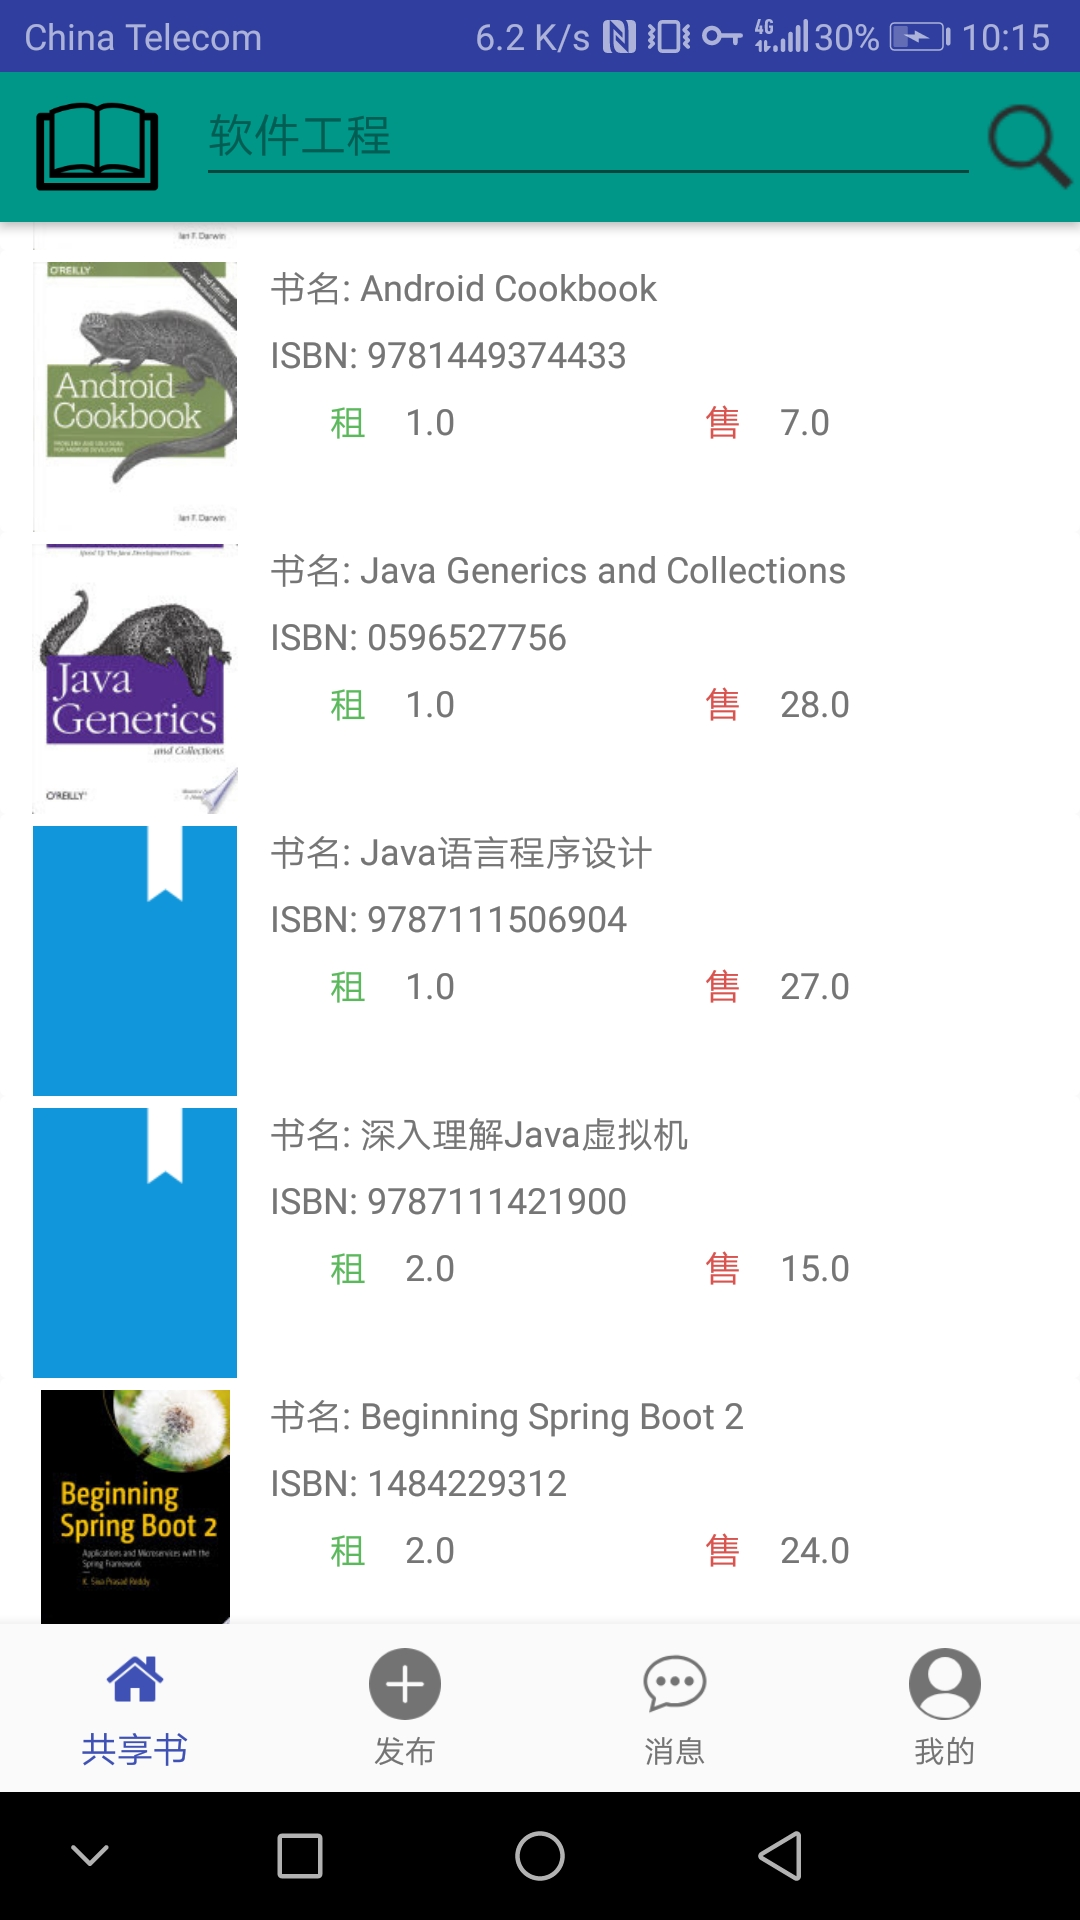
\includegraphics[scale=0.09]{Chapters/UI/book_list.jpg}
		\caption{客户端首页}
		\label{main_ui}
	\end{figure}

	导航栏是 App 的主要功能入口,导航栏有四个选项:共享书,发布,消息,我的。共享书对应 App 的主页,发布对应发布
	选项,消息对应最近联系人页面,我的对应与用户相关的页面。

\cref{self_intro}显示了个人主页,这里是与用户个人相关的页面,包括我的钱包,我的订单,我的发布,清除缓存 ,退出登录等。

\begin{figure}[h]
	\centering
	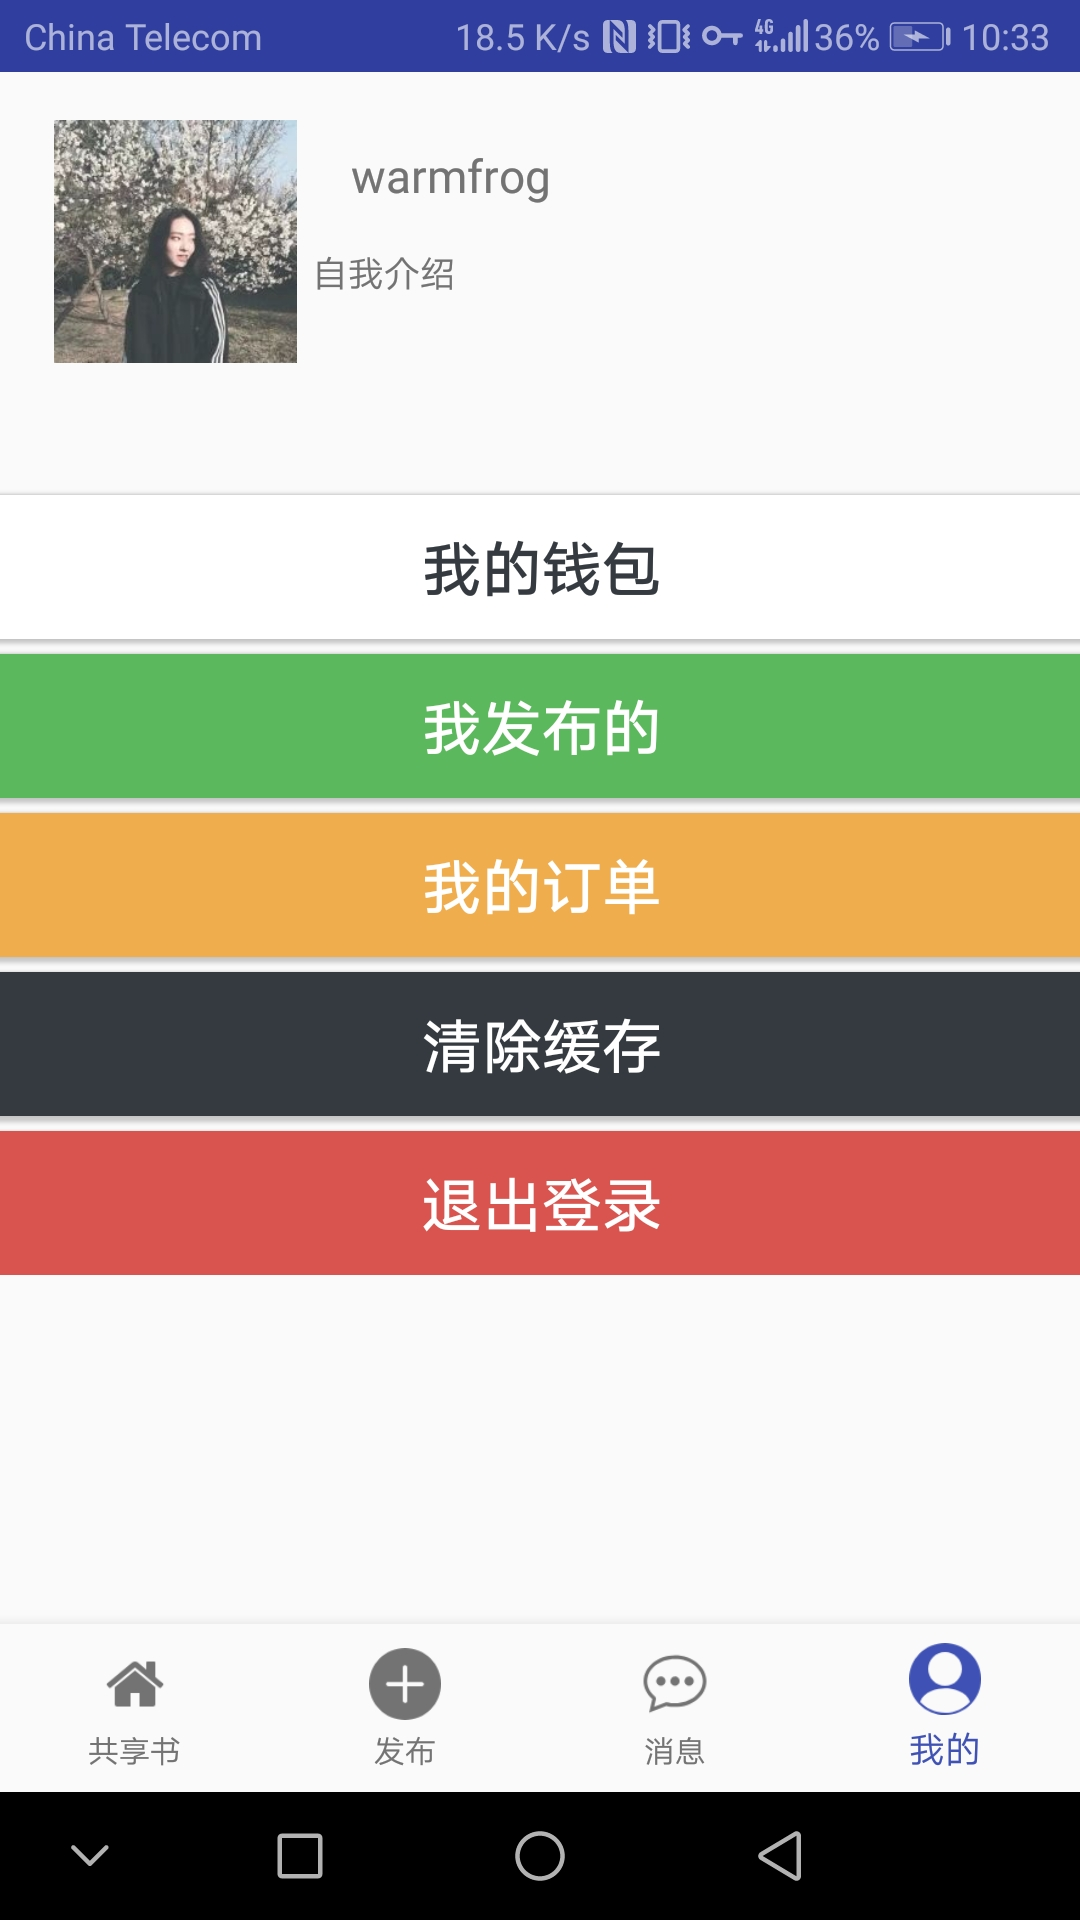
\includegraphics[scale=0.09]{Chapters/UI/self_intro.jpg}
	\caption{个人主页}
	\label{self_intro}
\end{figure}

\cref{unlogin}是用户未登录时进入点击我的导航栏时进入的页面,提示用户进行登录。

\begin{figure}[h]
	\centering
	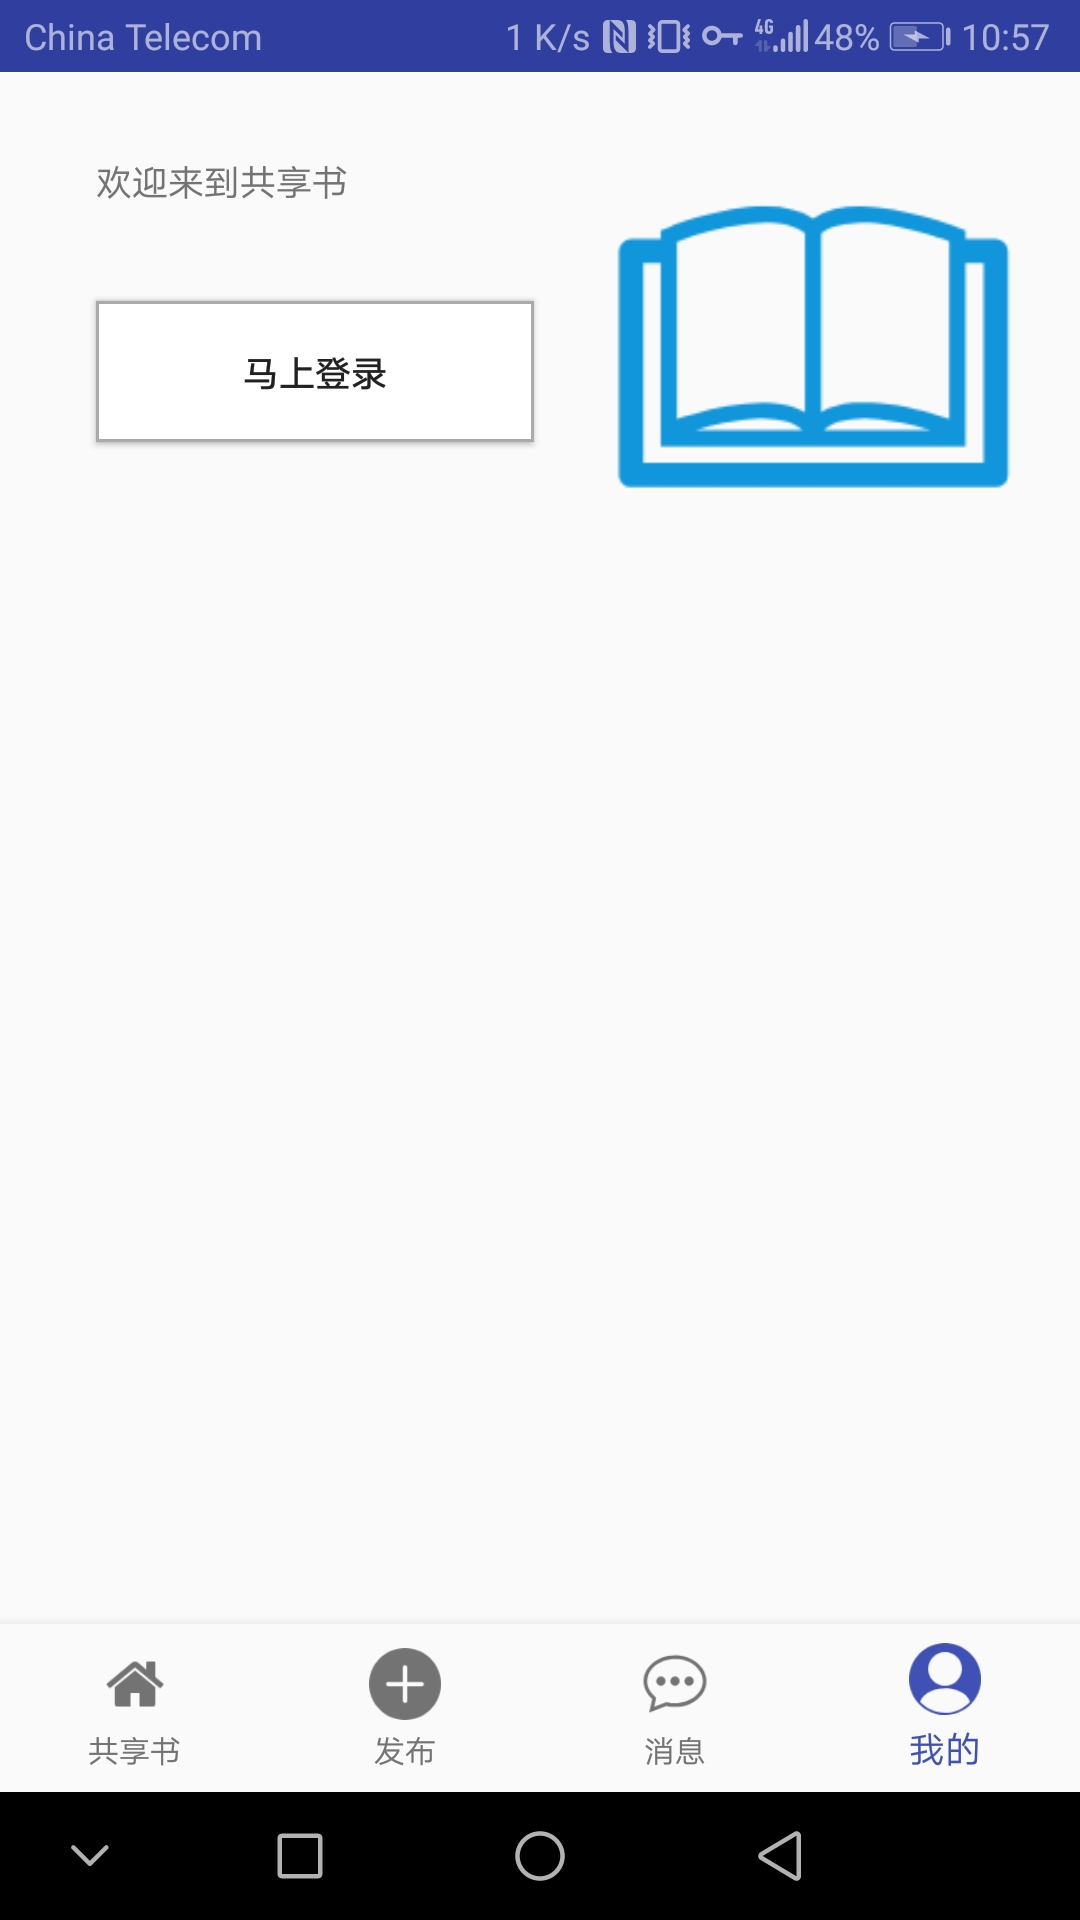
\includegraphics[scale=0.09]{Chapters/UI/unlogin.jpg}
	\caption{用户未登录}
	\label{unlogin}
\end{figure}

\subsection{用户模块}
\subsubsection{登录功能}
用户输入用户名或者注册邮箱和密码,点击是否记住账号和是否记住密码,当记住账号的复选框被勾选
时,用户账号会被记录到 Android 本地文件中;当记住密码的复选框被勾选时,用户密码也会保存到本地文件中。
用户点击登录,如果用户名不存在,将提示“用户名不存在,请注册”,如果密码不对,将提示账号或密码错误。
如果用户登录成功,则进入个人主页面。

\cref{login}是用户登录界面,用户通过输入注册时的用户名或者邮箱进行登录,如果密码不正确,或用户不存在,将提示用户重新登录或者注册。

\begin{figure}[h]
	\centering
	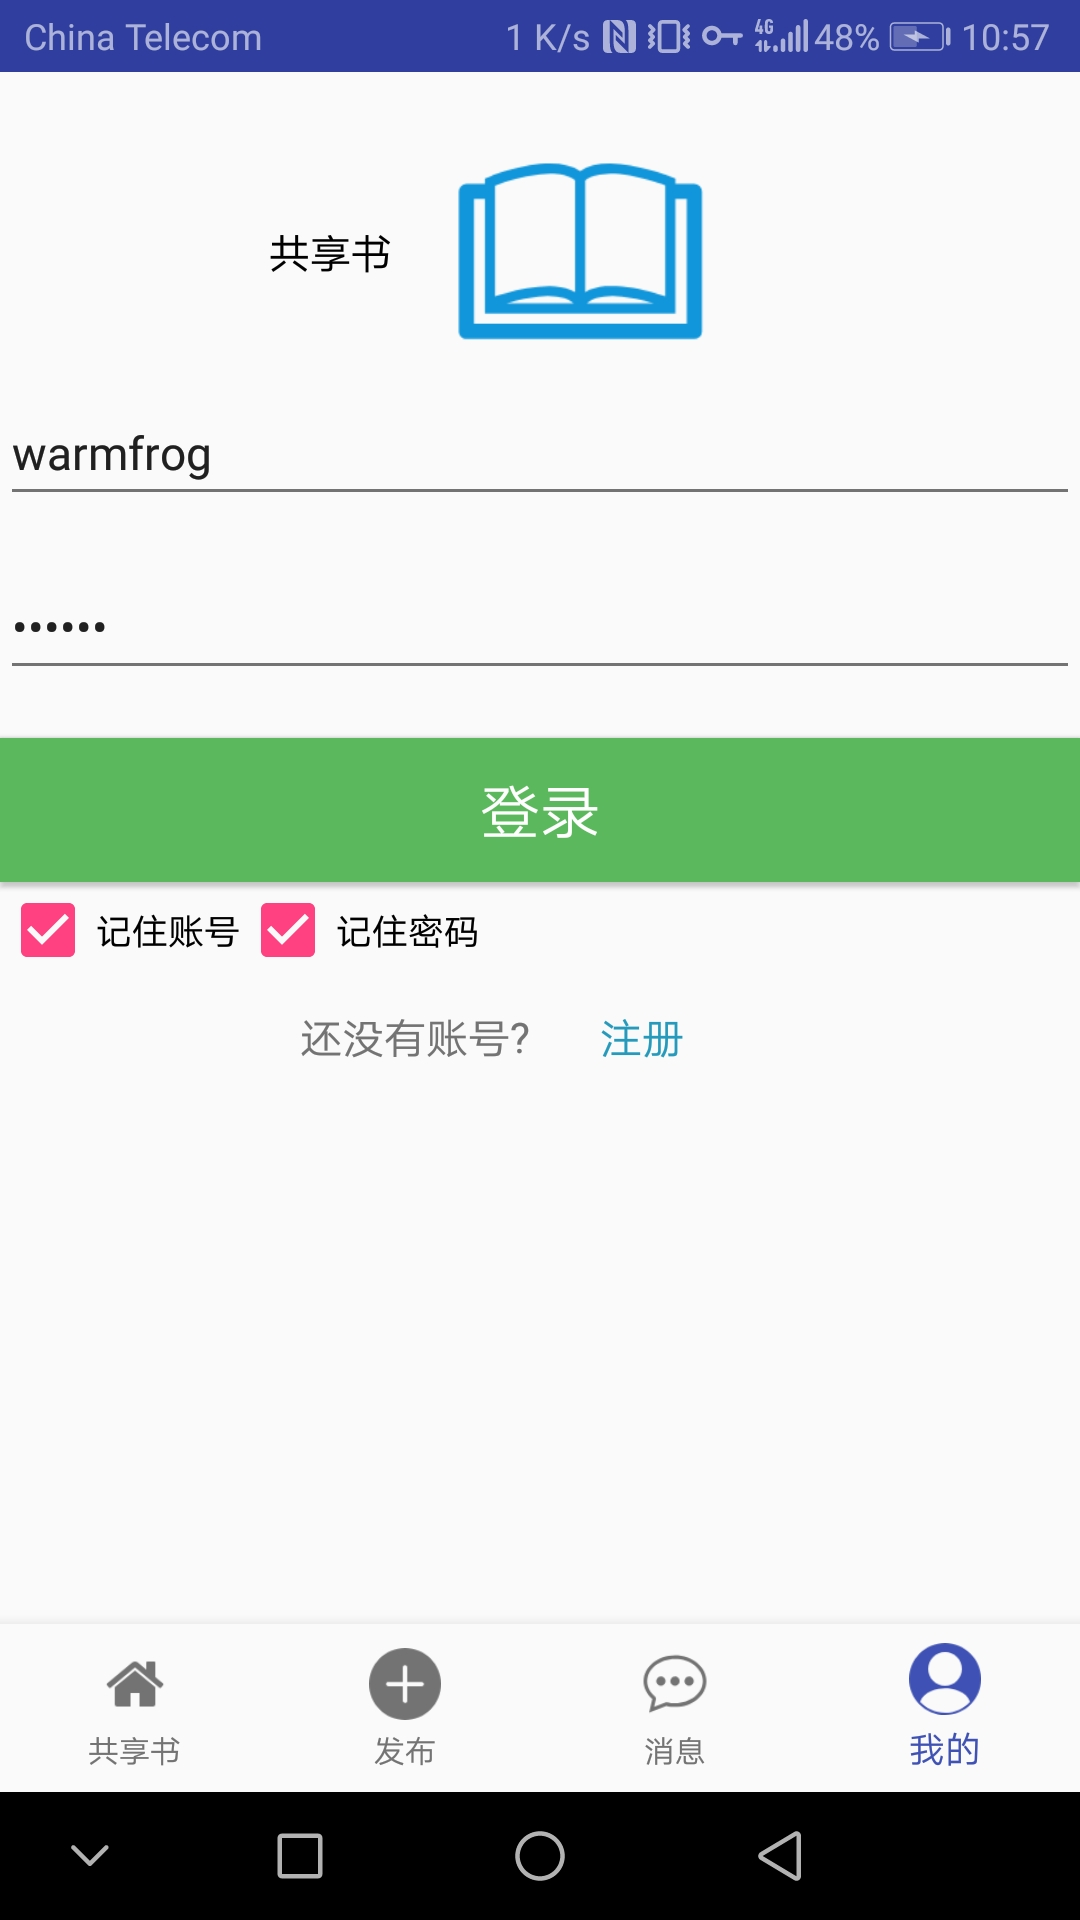
\includegraphics[scale=0.09]{Chapters/UI/login.jpg}
	\caption{登录}
	\label{login}
\end{figure}



\subsubsection{注册功能}
\cref{register}是用户注册页面,用户在该页面输入用户名,邮箱,密码等信息注册。
如果用户已存在,将提示用户,该账号已存在。

\begin{figure}[h]
	\centering
	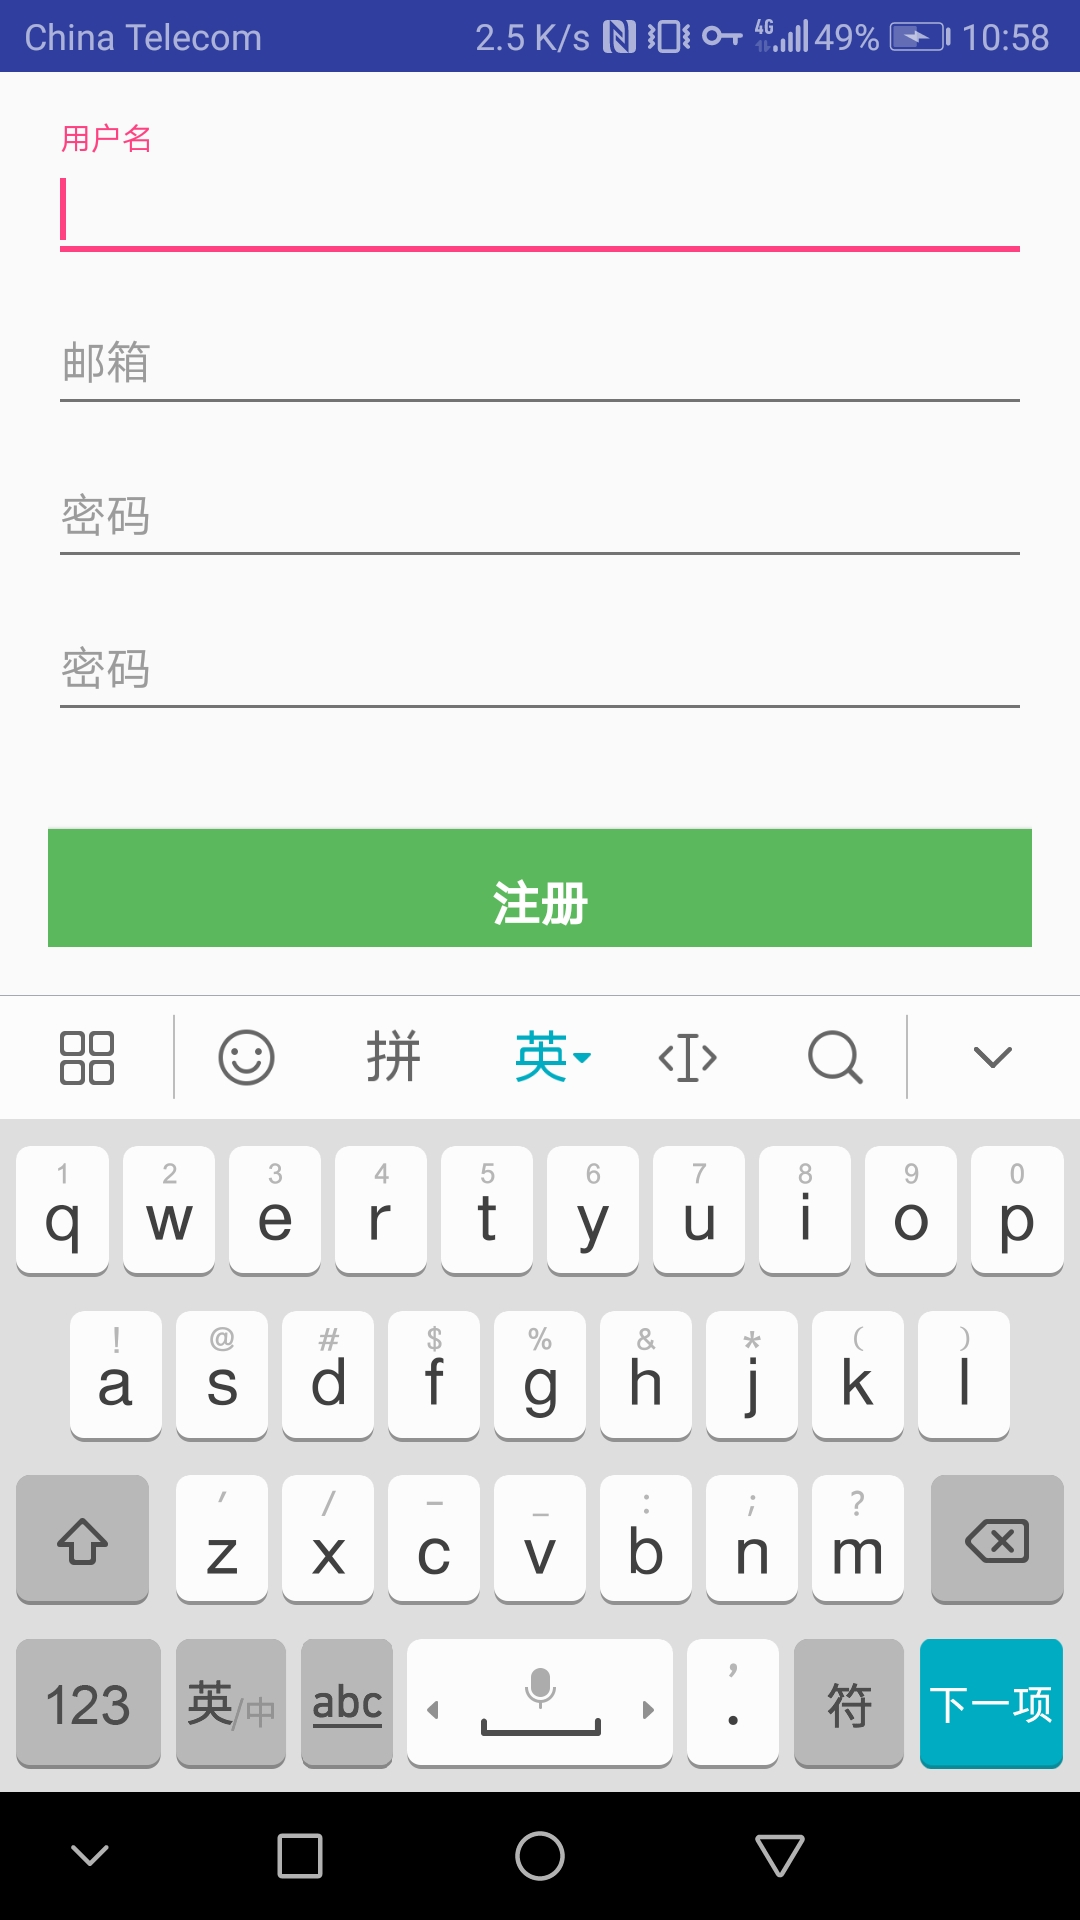
\includegraphics[scale=0.09]{Chapters/UI/register.jpg}
	\caption{注册}
	\label{register}
\end{figure}

用户进入登录界面,如果该用户没有账户,则可点击下方的提示注册按钮,进入注册页面。
用户在该页面输入用户名,邮箱,密码,确认密码信息。如果用户名或邮箱已经注册,将提示
该用户名或邮箱已经注册,请用户更换用户名或者登录。用户名和邮箱是绑定且唯一的。一个
邮箱只能注册一个账号。用户输入密码和确认密码,如果两次输入不一致,则提示用户两次输入
的密码不一致,请重新输入。




\subsection{发布图书}
用户点击发布图书,通过弹出的对话框,有两个选项。
一种方式是扫描条形码,用户点击该选项,将打开
一个 Activity 页面,该页面打开一个相机,中心是一个方形条形码区域,用户对准图书的条形码
区域,通过扫描,获取图书 ISBN;
另一个方式是手动输入图书的 ISBN。最终,用户将通过该 ISBN 获取该
书的所有相关信息,如果并未获取到该图书信息,下方弹出提示,未查询到该书信息,如果成功查询到该
书信息,将打开一个用户图书发布页面,该页面上方显示该书的详细信息,包括图书封面图片,图书 ISBN 信息,
图书的名称,图书的作者以及图书的出版时间信息,下方是用户自行补充的发布信息:包括租赁价格,出售价格
等。平台假定用户上传的图书都是可以租出和出售的。可选的,用户还可以输入相关描述信息,可以是图书推荐或者
图书使用情况。最终点击下方的发布按钮,完成图书发布。

用户点击发布时,有两种方式发布图书:一种是通过手机扫描图书条形码,获取图书 ISBN 获取
图书信息,一种是通过手动输入图书 ISBN。如\cref{release}所示。

\begin{figure}[h]
	\centering
	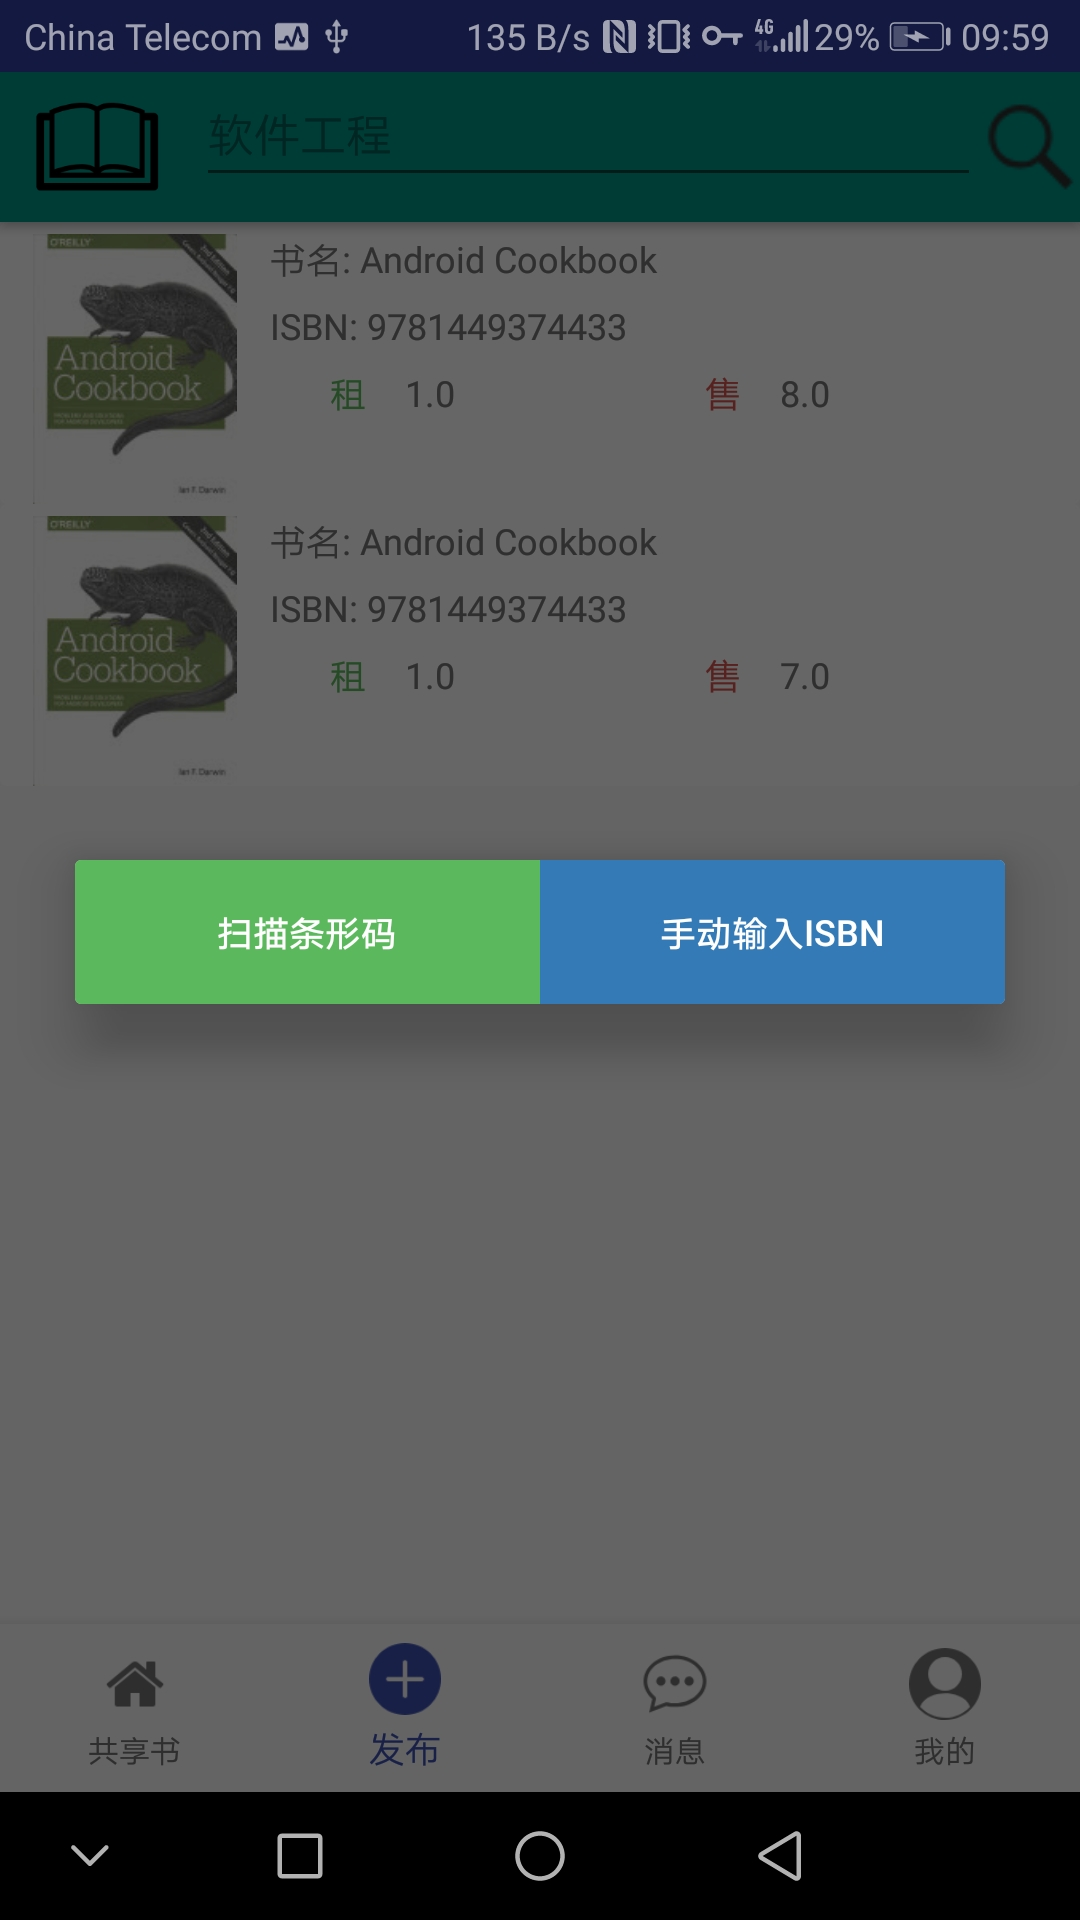
\includegraphics[scale=0.09]{Chapters/UI/release.jpg}
	\caption{点击发布}
	\label{release}
\end{figure}

\cref{scan}是用户点击发布后,选择扫描条形码时进入的页面,在该页面调用 Android
相机,扫描条形码,解析条形码,获取图书的 ISBN 信息,将 ISBN 发送到服务器,获取相应的图书信息。

\begin{figure}[h]
	\centering
	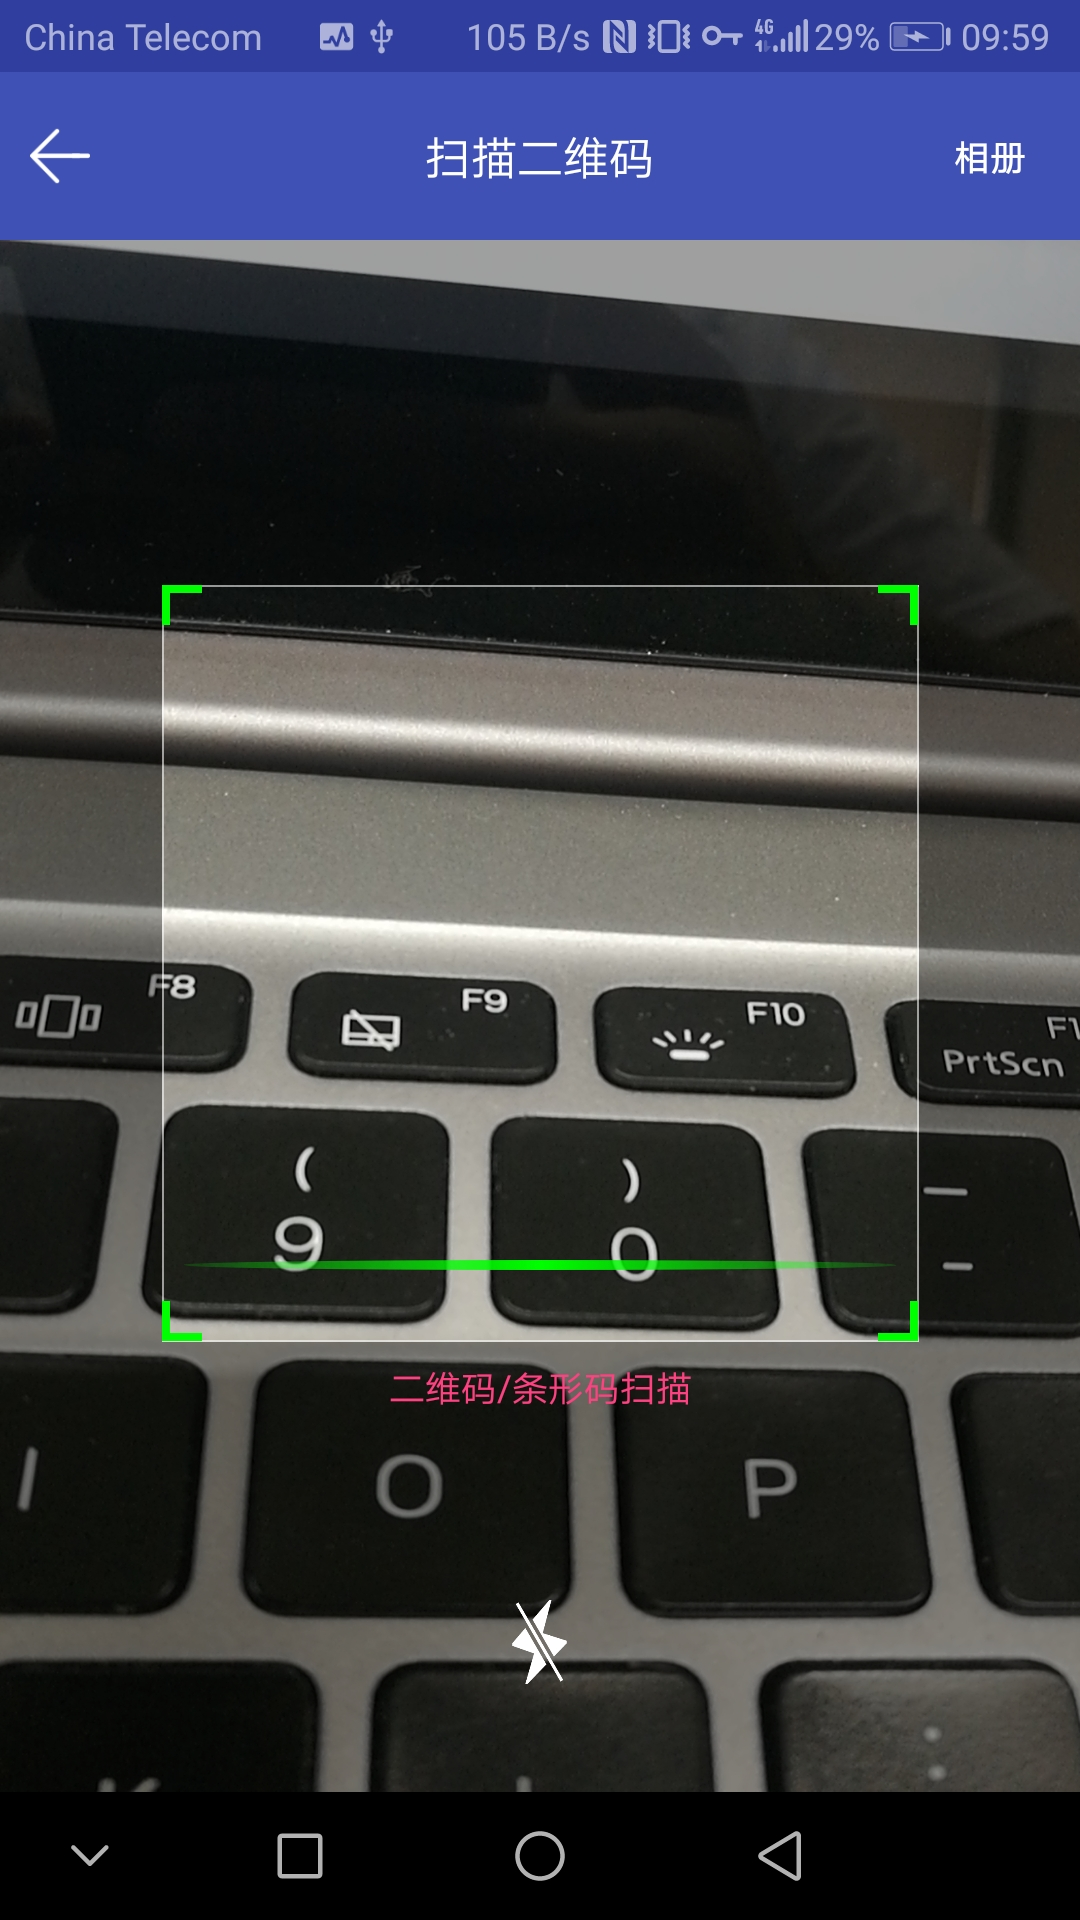
\includegraphics[scale=0.09]{Chapters/UI/scan.jpg}
	\caption{扫码图书条形码}
	\label{scan}
\end{figure}

\cref{input_isbn}是用户点击发布后,选择手动输入 ISBN 时进入的页面,用户在编辑栏手动输入图书的 ISBN 信息,发送到服务器来获得图书信息。

\begin{figure}[h]
	\centering
	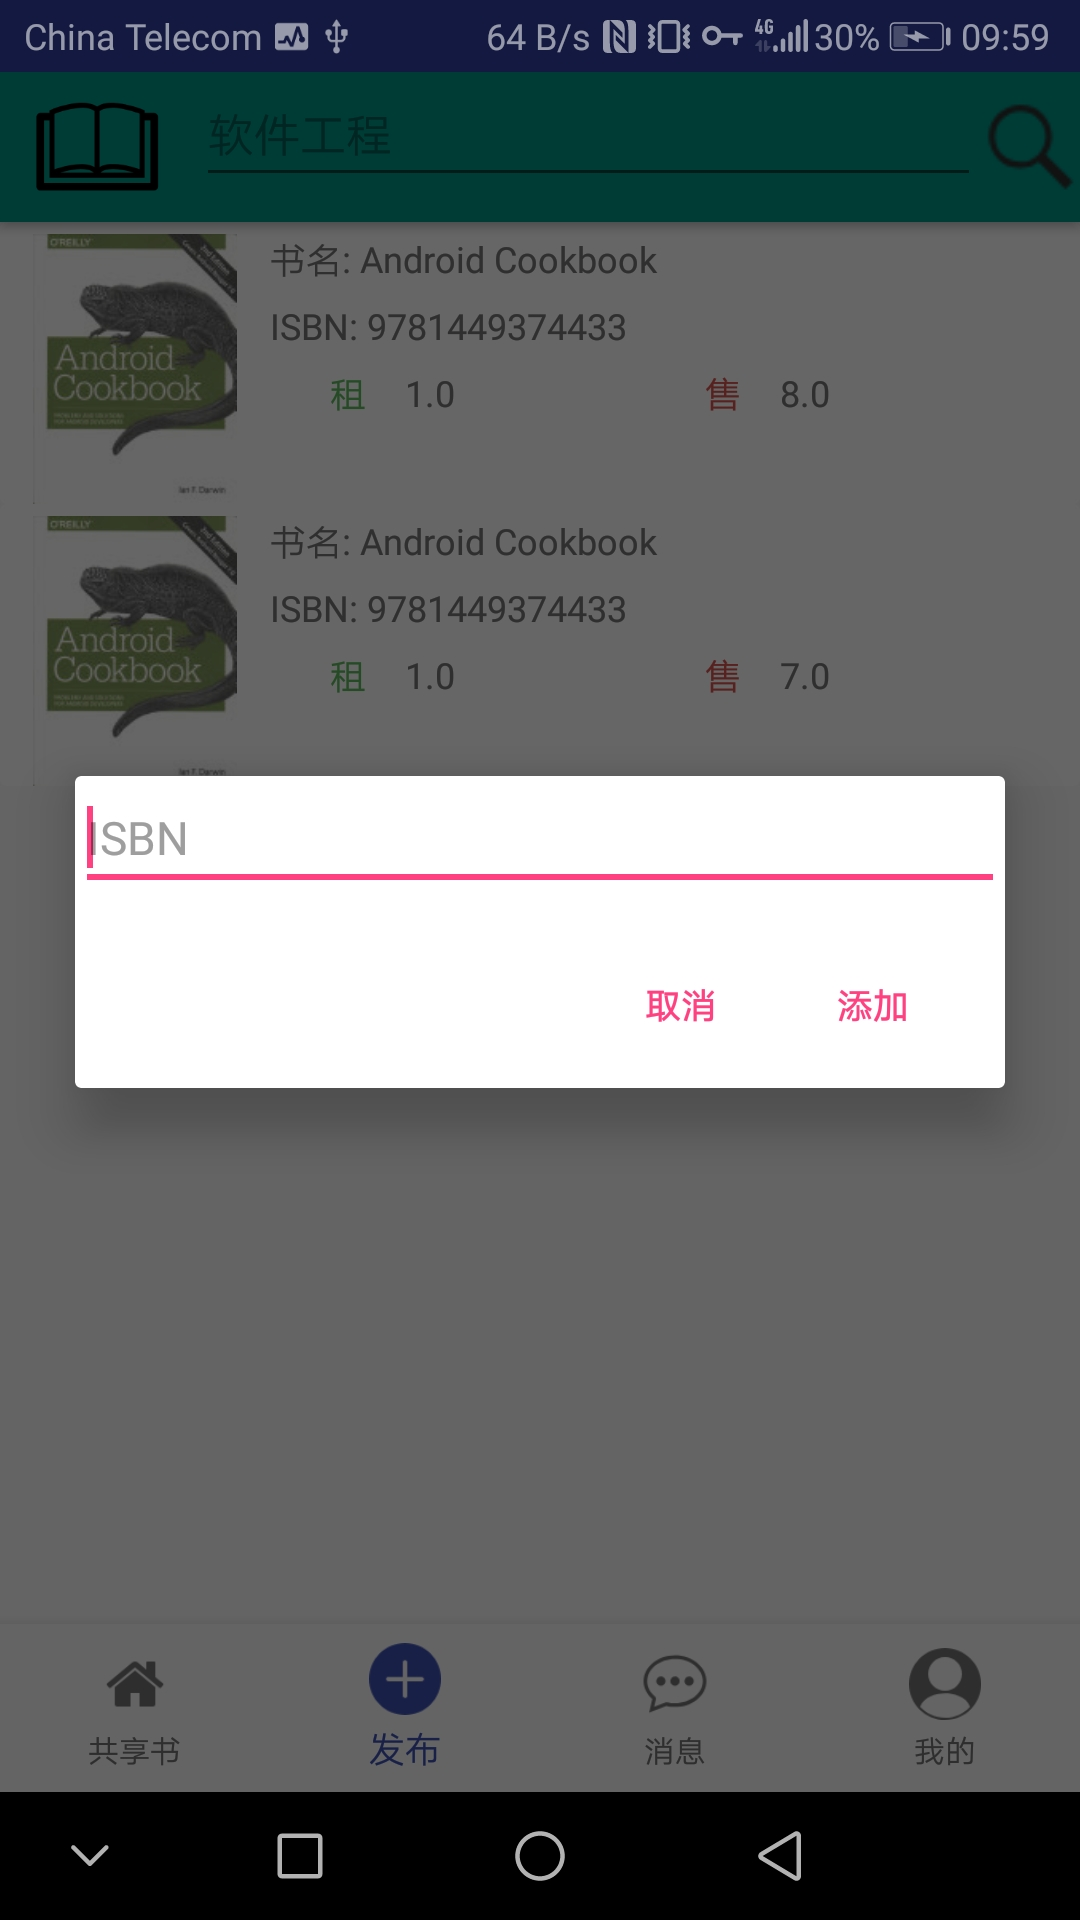
\includegraphics[scale=0.09]{Chapters/UI/input_isbn.jpg}
	\caption{手动输入图书ISBN}
	\label{input_isbn}
\end{figure}


\cref{release_from}是发布页面,用户点击发布,并从服务器获取到图书信息后,将进入此界面,用户进一步补充
相关的发布信息,如价格,个人平台或者描述等(可选),然后点击下方发布按钮进行发布。

\begin{figure}[h]
	\centering
	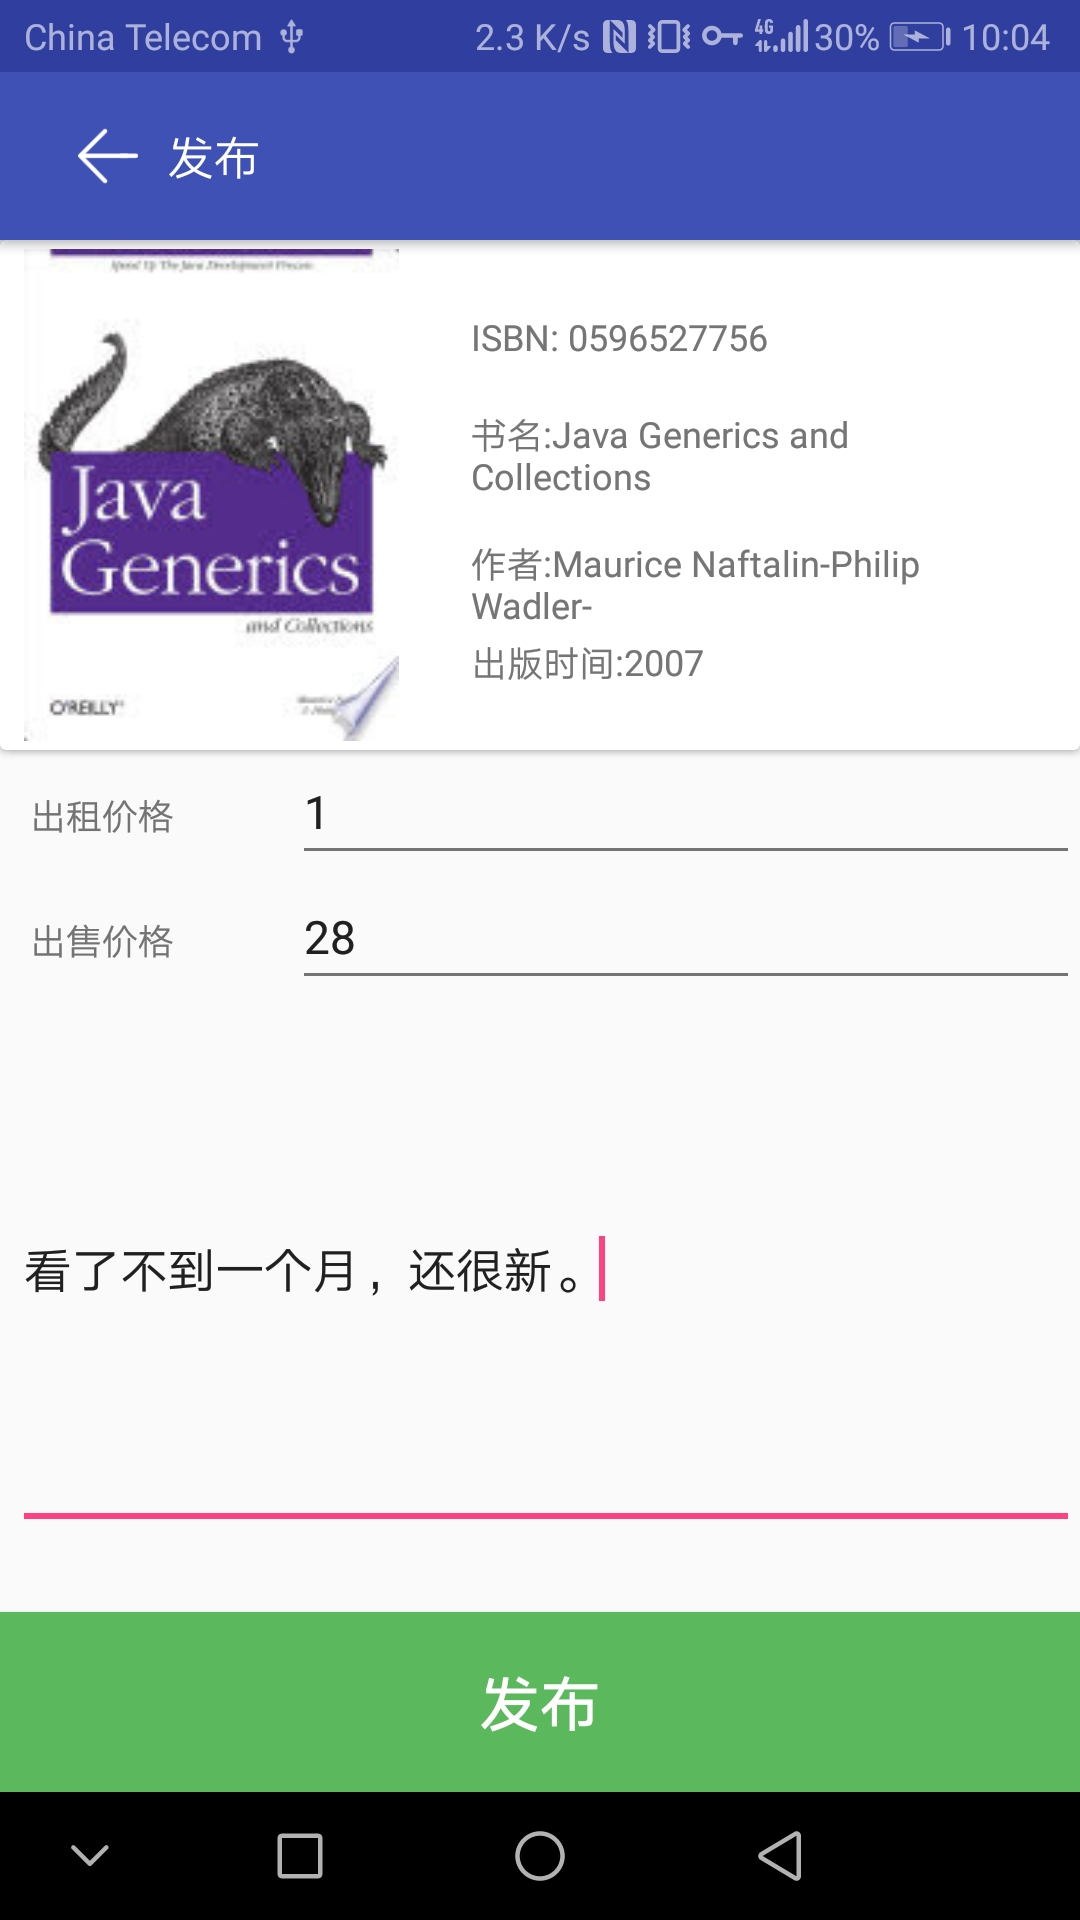
\includegraphics[scale=0.09]{Chapters/UI/release_form.jpg}
	\caption{补充发布信息}
	\label{release_from}
\end{figure}

\subsection{浏览图书}
用户打开主界面,主界面显示目前已加载的已发布的图书列表,列表的每一项包含少量的信息,包括图书封面,图书名,图书
ISBN,图书的租赁价格,图书的购买价格等信息。用户下拉,图书将持续加载,直至加载完所有图书。用户可以
通过点击某一项,查看自己感兴趣的图书的详细信息,并进行下一步操作。

\subsection{查看图书}

用户对某本书感兴趣,点击图书项后,打开一个新的 Activity 页面,该页面将显示该书的详细信息,上面是图书的基本信息,
包括图书封面,图书 ISBN,图书作者,图书名,出版时间,租赁价格,出售价格。中部是用户发布时的自行描述信息,下面
是图书的简介,最底部是两个选项,租赁、购买和聊一聊。用户点击租赁或购买时,会进入一个新的创建订单 Activity 页面,如\cref{order}所示。

\begin{figure}[h]
	\centering
	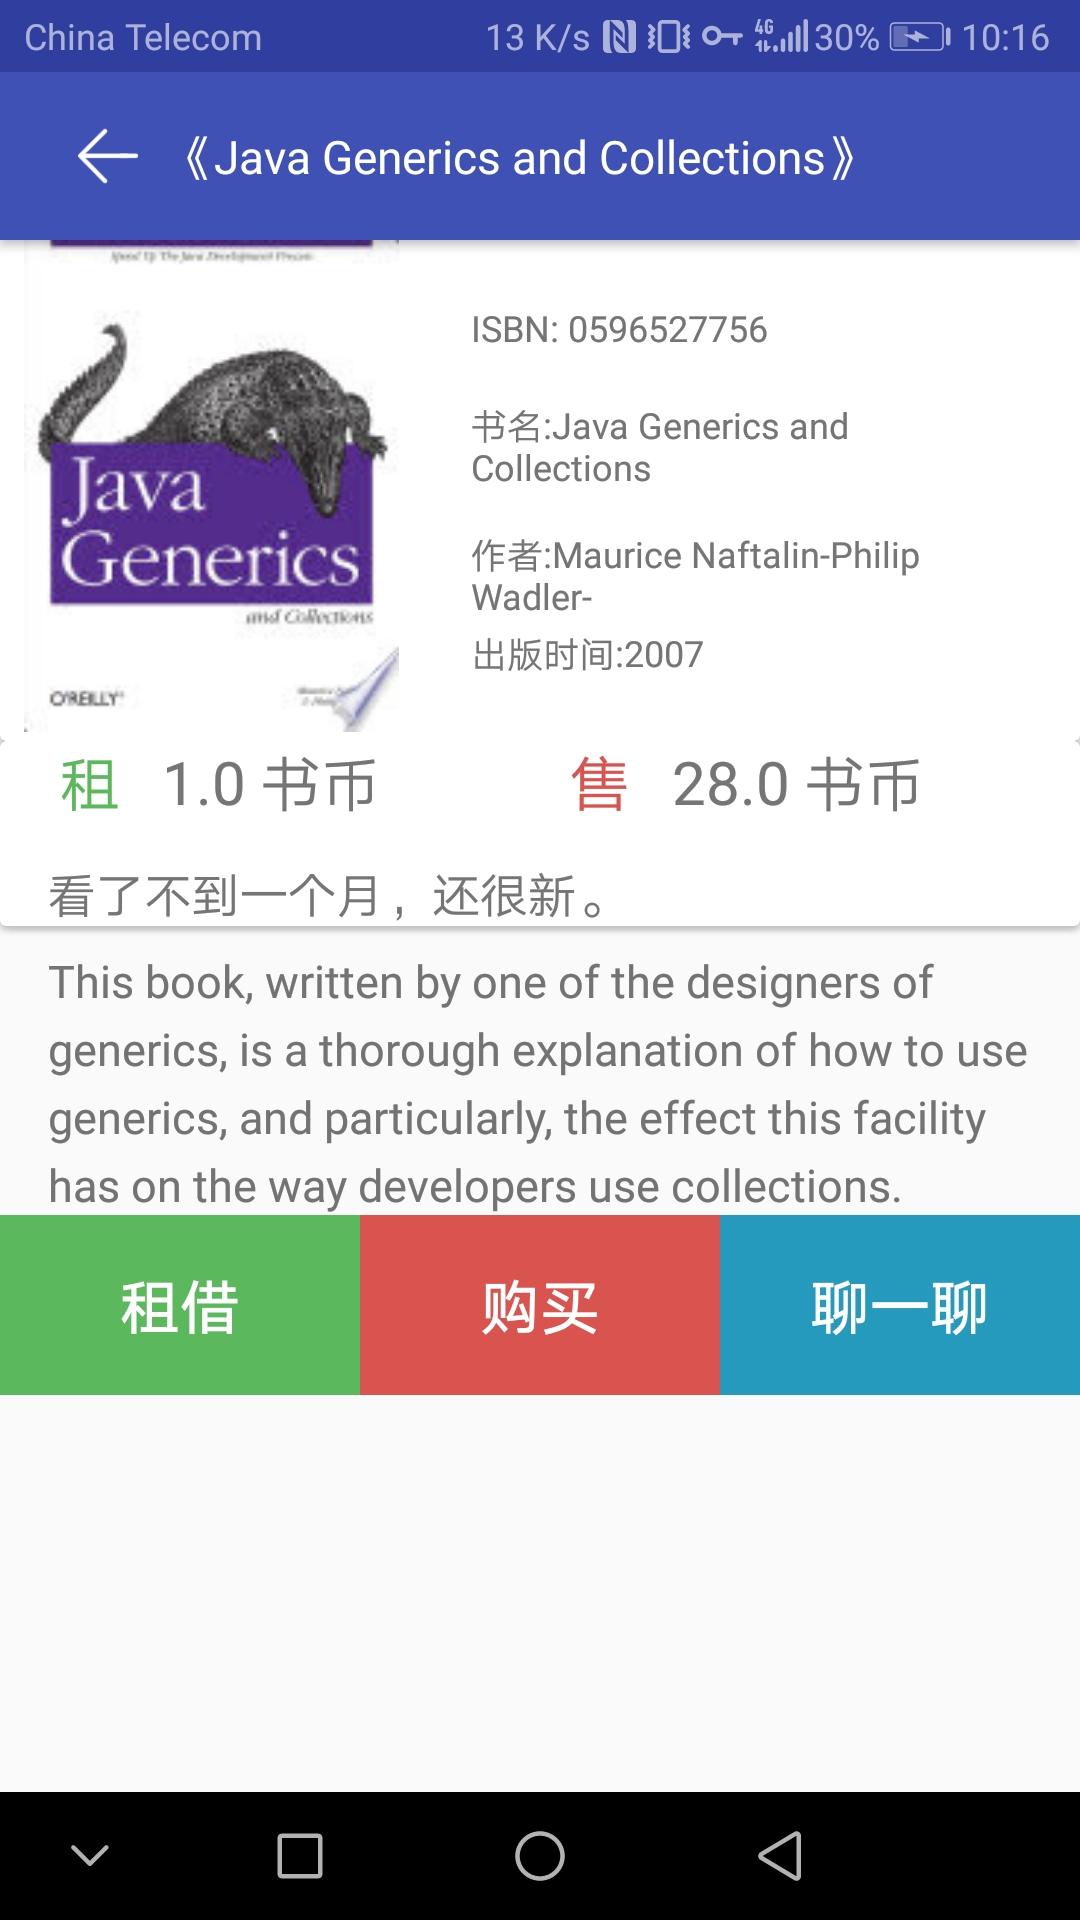
\includegraphics[scale=0.09]{Chapters/UI/ubook_info.jpg}
	\caption{图书详情}
	\label{ubook_info}
\end{figure}

当用户点击聊一聊时,打开一个聊天 Activity 界面,用户可以与图书主人聊天沟通,如\cref{talk}所示。

\cref{ubook_info}是图书详情信息,当用户点击图书某项时,会进入该页面,并显示图书详情信息,包括书名,ISBN,作者,描述等信息。

\begin{figure}[h]
	\centering
	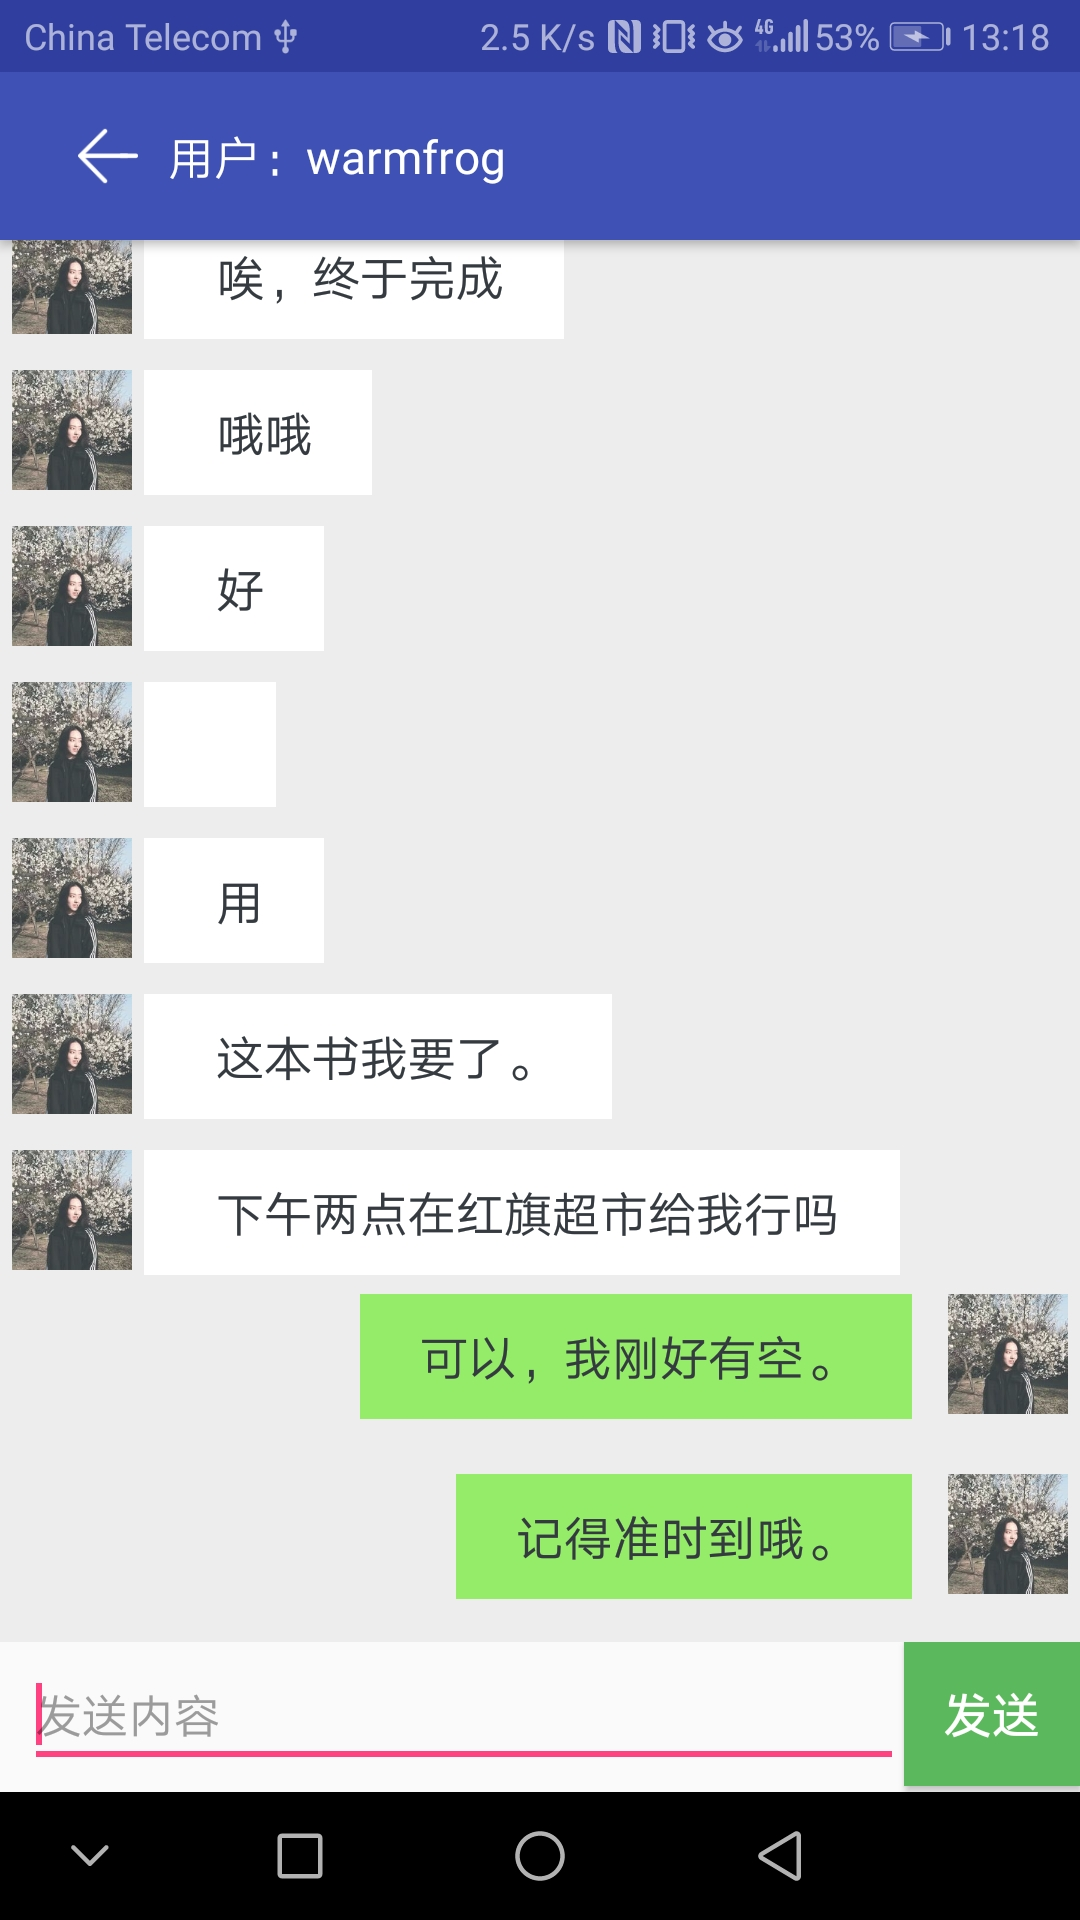
\includegraphics[scale=0.09]{Chapters/UI/talk.jpg}
	\caption{聊天沟通界面}
	\label{talk}
\end{figure}

\subsection{租赁购买图书}
\cref{order}是下单页面, 用户对某本书进行借阅或者购买时,会打开创建订单页面,上面是要下单的图书信息,封面,ISBN,作者,发布时间,下面是
从服务器获取的生成订单的信息,包括订单号,订单金额,订单时间,订单状态,订单类型等信息,最下面是要支付的总额
和立即支付按钮。用户点击支付,如果用户账户余额大于或者订单金额,将从用户账户扣除订单金额,并打开新的页面,提示用
户支付成功。否则,在新的页面提示用户支付失败。
相关的信息,会获取到服务器生成的订单号,

\begin{figure}[h]
	\centering
	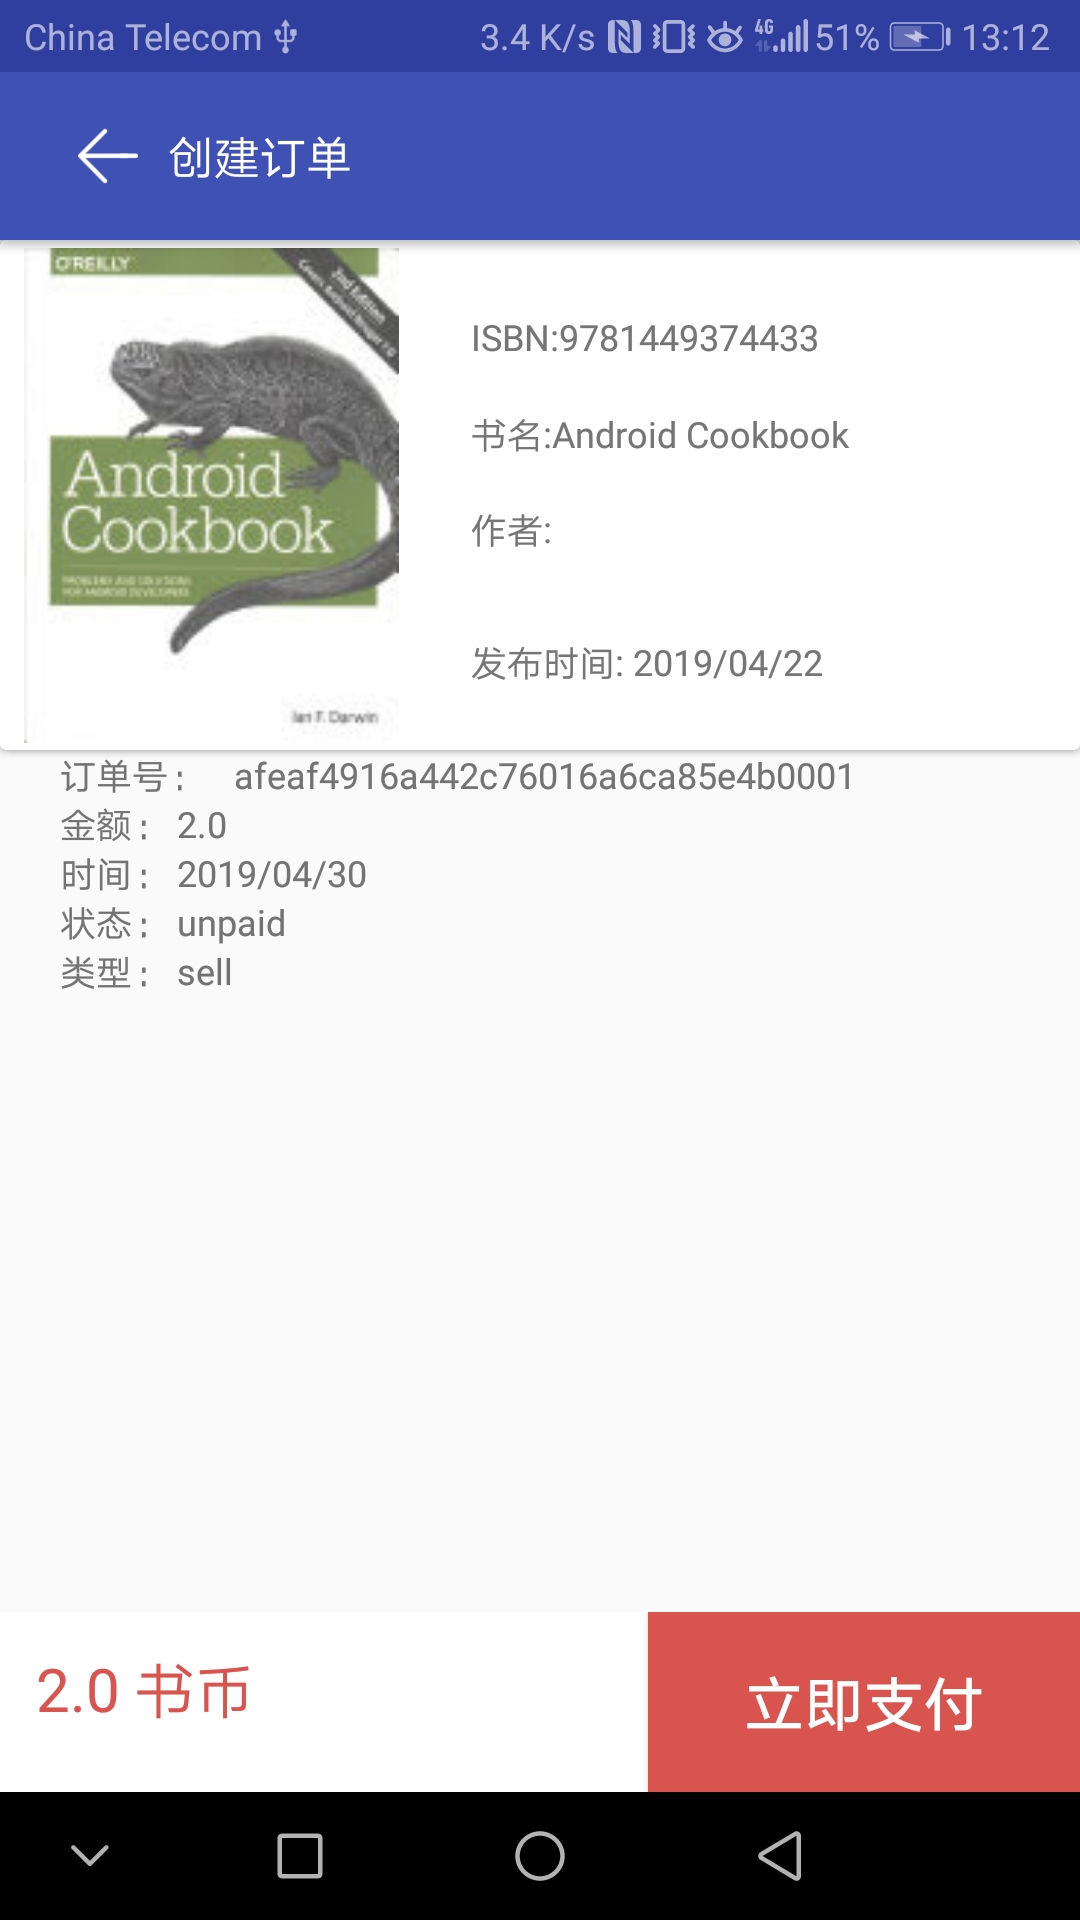
\includegraphics[scale=0.09]{Chapters/UI/order.jpg}
	\caption{下订单}
	\label{order}
\end{figure}

\subsection{管理图书}
用户在下方的导航栏点击我的-我发布的,进入我的发布页面。这也是一个图书列表,仅仅包含了当前登录用户的发布图书,每
一项包含图书封面,图书名,图书租赁价格,购买价格,发布时间和一个复选框。当用户点击某一项进入图书详情页,图书详情
页面包含详细的图书信息,包括图书封面,图书 ISBN,图书名,图书作者,出版时间,租赁价格,购买价格,用户自定义描述信息,
图书简介内容。页面最上面的动作栏包含一个返回按钮,图书的标题和帮助按钮。用户点击返回,将返回到图书列表页面。用户点击
帮助按钮,将在下方弹出帮助信息,提示用户选择要删除的项,并删除。帮助信息在两秒后自动消失。用户点击某一项的复选框时,
下方将弹出一个提示信息,提示用户是否删除该图书,如果用户点击删除,则将删除该书。如果用户无操作,提示信息在两秒后自行消失。

\cref{myubook}是我的发布页面。当用户在个人主页点击我的发布时进入该页面,显示该用户已发布的书籍列表。

\begin{figure}[h]
	\centering
	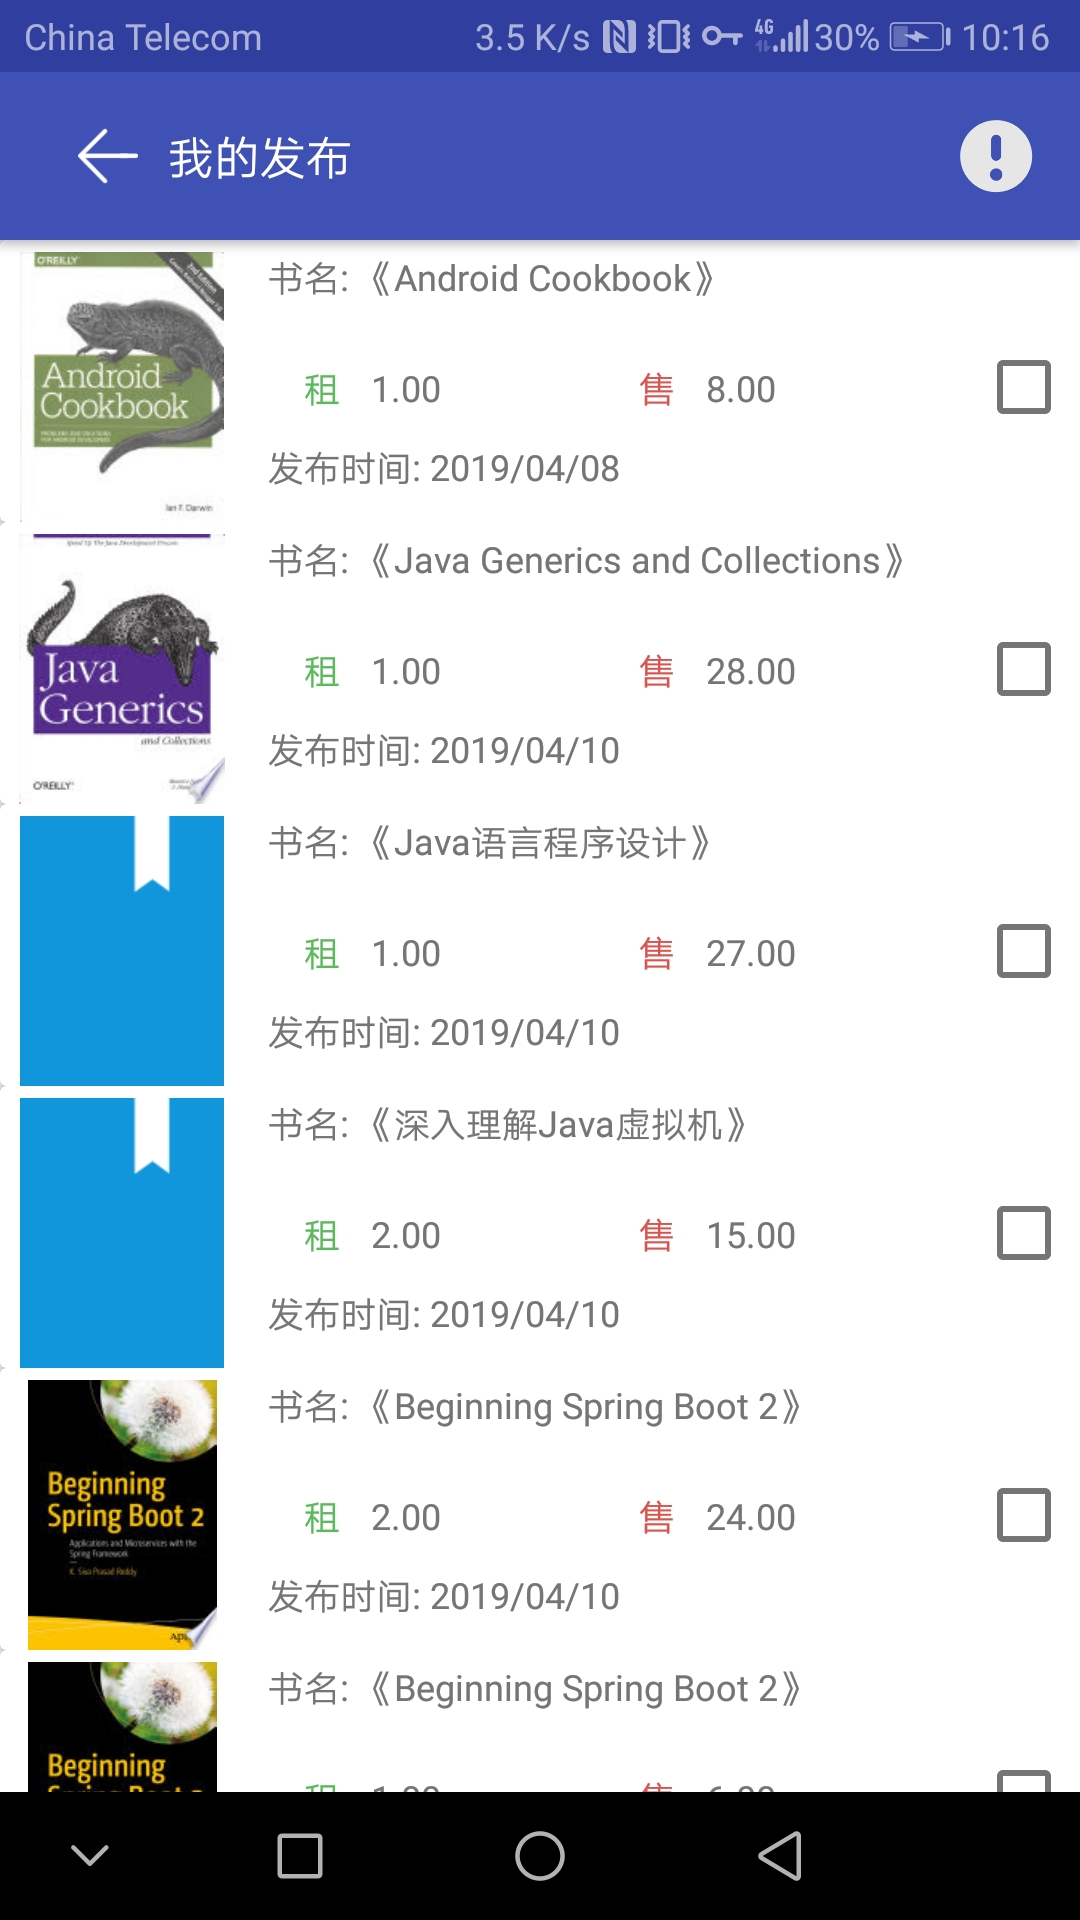
\includegraphics[scale=0.09]{Chapters/UI/myubook.jpg}
	\caption{我的发布}
	\label{myubook}
\end{figure}

\subsection{订单管理}
用户在下方的导航栏,我的-我的订单,进入我的订单页面。这里将显示用户所有的订单信息。订单页面动作栏显示一个返回按钮和标题
我的订单。用户点击返回按钮,将返回我的个人主页。订单页面包含订单列表。每一项包含订单的详细信息,分为三个区域上中下。上区域
最上面显示该订单中图书的拥有者信息,订单的状态。上区域的下面包含该订单中的图书信息,包含图书封面,图书标题,图书 ISBN。中
区域包含订单信息,包含订单号,订单金额,下单时间,订单状态,订单类型。下区域是两个按钮,包含对订单的操作。

\begin{figure}[h]
	\centering
	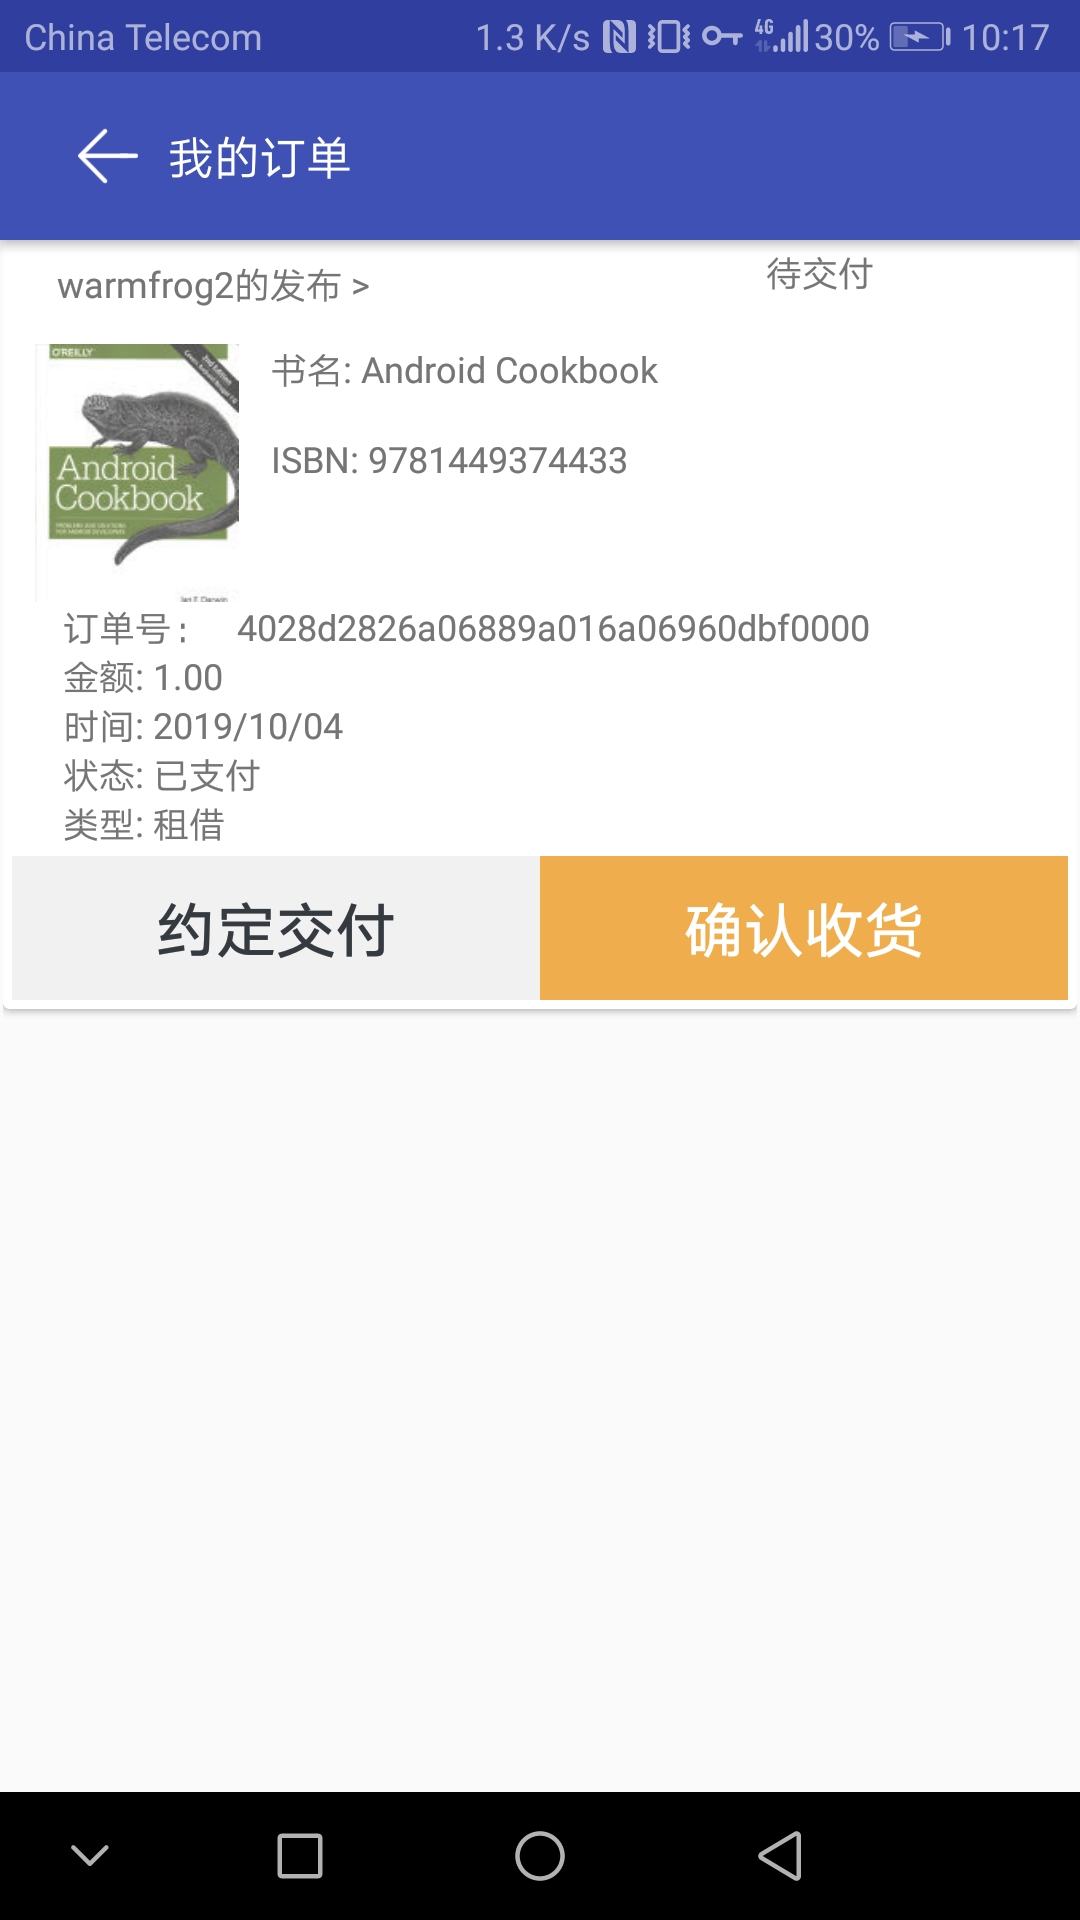
\includegraphics[scale=0.09]{Chapters/UI/unrecieved_order.jpg}
	\caption{我的订单}
	\label{unrecieved_order}
\end{figure}

订单包含了不同状态和类型。订单的类型包括租赁类型和购买类型。状态包括未支付状态,已支付状态,已完成状态和关闭状态。

用户下单时,租赁方式对应订单的租赁类型,购买对应订单的购买类型。用户下单后,订单为未支付状态,此时用户可以取消订单和支付订单。
用户支付订单后,订单变为已支付待交付状态,用户可以确认收获。消费者确认收货后,用户变成已完成状态,用户可以选择删除
订单信息。用户取消订单后,订单变为关闭状态,用户可以选择删除订单。

\cref{unrecieved_order}是我的订单页面。用户在个人主页点击我的订单时进入该页面。
显示用户所有的订单页面,用户可以对
订单进行状态的改变或者删除操作。



\subsection{钱包管理}
用户在下方的导航栏点击我的-我的钱包,进入我的钱包页面。我的钱包头部的动作栏包含一个返回按钮和标题余额。下方是提示信息余额账户
(书币),再下面是用户的账户余额,背景色为淡蓝色。下方是提示信息,提示用户如何获得书币。

目前书币获得策略设定为新注册用户获得两个书币,之后,用户每上传一部图书,都将获得一个书币。

\cref{balance}是我的钱包页面。当用户在个人主页点击个人钱包时进入该页面,该页面显示账户余额信息。

\begin{figure}[h]
	\centering
	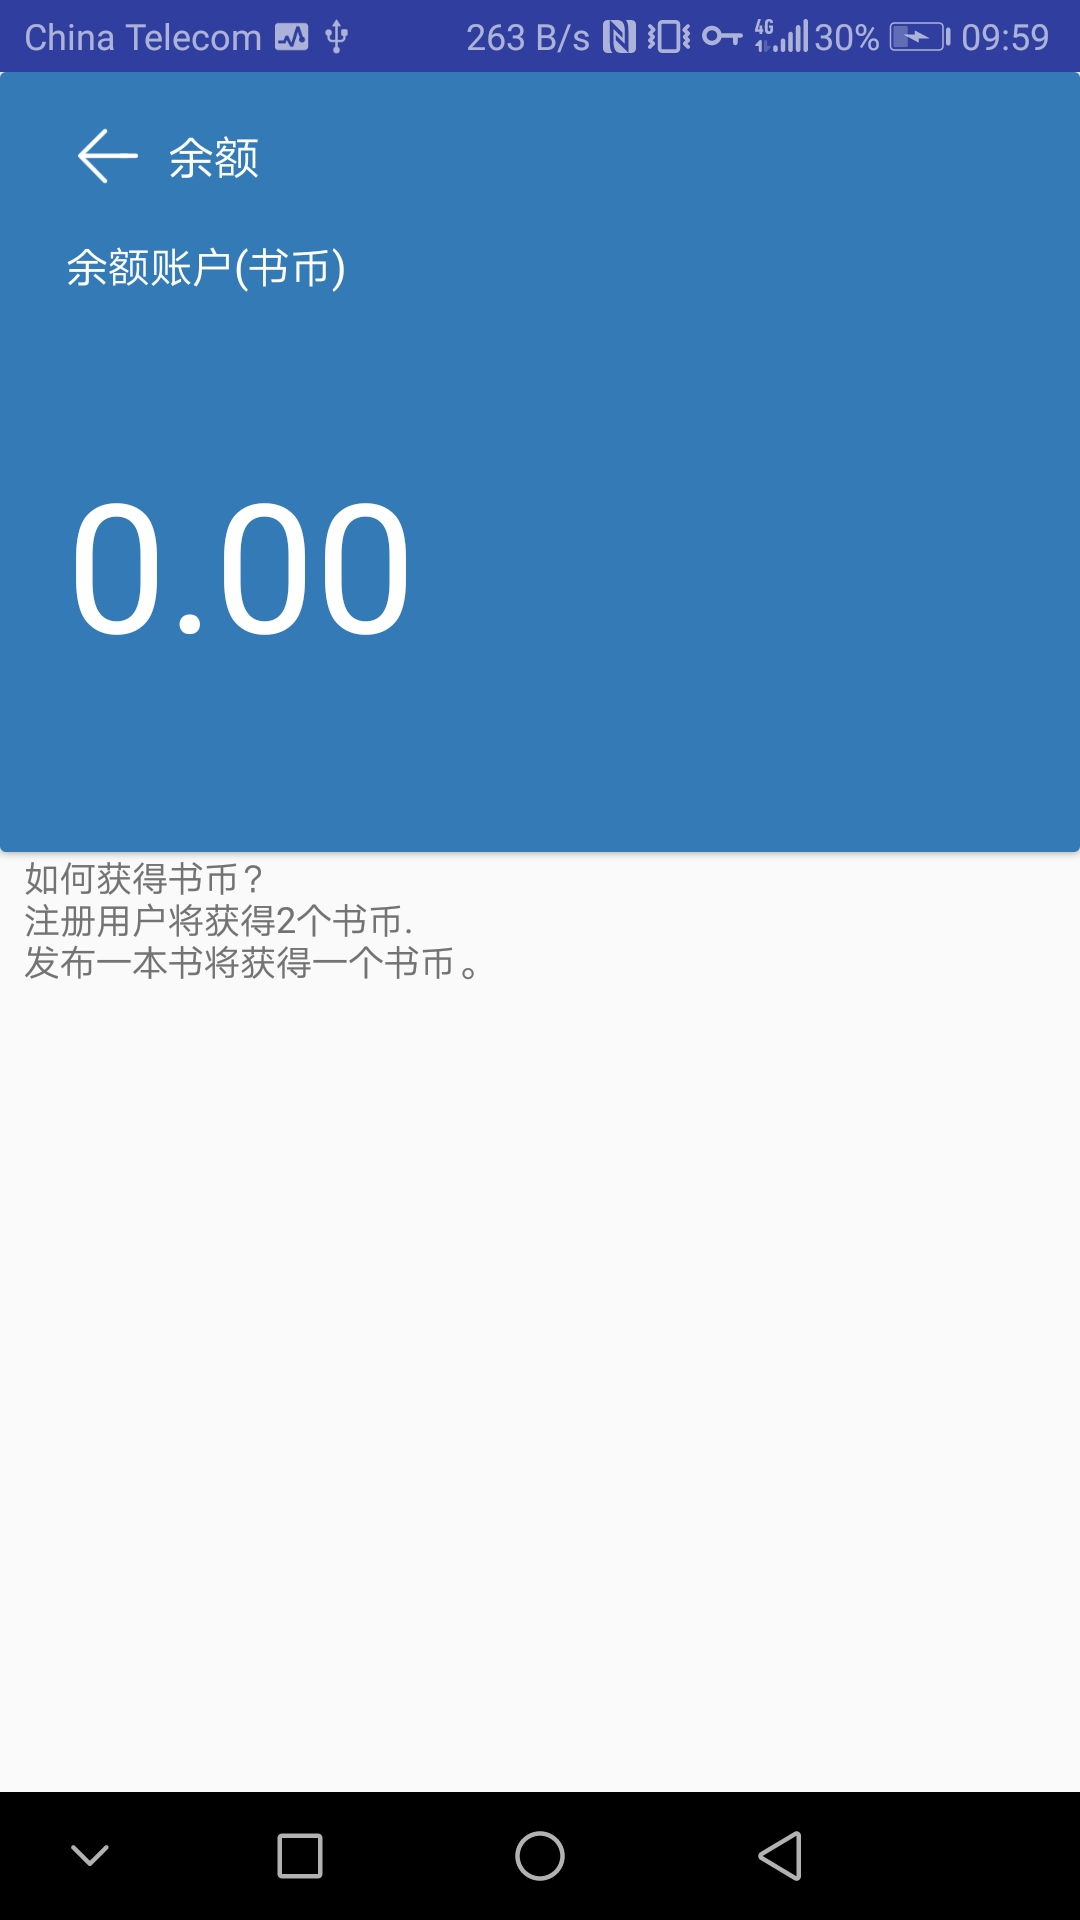
\includegraphics[scale=0.09]{Chapters/UI/balance.jpg}
	\caption{我的钱包}
	\label{balance}
\end{figure}

\subsection{清除缓存}
用户点击我的-清除缓存,将删除当前应用本地文件信息,用户属性信息,和本地 Sqlite 数据库所有数据。

\subsection{退出登录}
用户点击我的-退出登录,将删除用户本地属性文件中已登录的 token 信息。并进入默认的提示登录信息页面。之后,用户通过点击我的,只能
进入提示登录页面,用户只有登录后,才能进入个人主页。

\section{数据库设计}
		
\begin{enumerate}
	\item 用户表设计user
	
	\begin{table}[h]
		\centering
		\caption{用户表设计user}
		\label{user_table}
		\begin{tabular}{ccccc}
			\toprule
			\textbf{字段名} & \textbf{数据类型} & \textbf{长度} & \textbf{其他}  & \textbf{备注} \\
			\midrule
			id  & int & 11 & 主键 & 用户ID \\
			username & varchar & 255 & unique & 用户名 \\
			create\_date & datetime & default & not null & 用户创建时间 \\
			email & varchar & 255 & unique & 用户邮箱 \\
			enabled & bit & 1 &  & 用户是否有效 \\
			password & varchar & 255 & not null & 加密后的用户密码 \\
			phone & varchar & 255 & unique & 用户绑定手机 \\
			\bottomrule
		\end{tabular}
	\end{table}

	\cref{user_table}是用户表,用户表包含用户 ID,用户名,用户创建时间, 用户邮箱 , enabled ,用户密码,用户手机等字段。
	用户 ID 为数据库自增;用户名为 unique 类型,表示不能重复;用户邮箱和手机同样为 unique,不能重复;enabled 表示用户是否
	有效;用户密码保存加密过的用户密码。

	\item 图书表gbook\$volume\_info设计
	
	\cref{gbook$volume_info_table}是图书详情表,包含自增 ID,购买连接,内容版本,内容描述,详情连接,语言版本,
	成熟度评分,页数,预览链接,出版类型,出版日期,子标题,标题等字段。
	\begin{table}[h]
		\centering
		\caption{图书表Gbook设计}
		\label{gbook$volume_info_table}
		\begin{tabular}{ccccc}
			\toprule
			\textbf{字段名} & \textbf{数据类型} & \textbf{长度} & \textbf{其他}  & \textbf{备注} \\
			\midrule
			id  & int & 11 & 自增主键 & ubook ID \\
			allow\_anon\_logging & bit & 1 & not null & "" \\
			canonical\_volume\_link & varchar & 255 & null & 购买连接 \\
			content\_version & varchar &255 & null & 内容版本 \\
			description & varchar & 4096 & null & 内容描述 \\
			info\_link & varchar & 255 & null & 详情连接 \\
			language & varchar & 255 & null & 语言版本 \\
			maturity\_rating & varchar & 255 & null & 成熟度评分 \\
			page\_count & bigint & 20 & null & 页数 \\
			preview\_link & varchar & 255 & null & 预览链接 \\
			print\_type & varchar & 255 & null & 出版类型 \\
			published\_data & varchar & 255 & null & 出版日期 \\
			subtitle & varchar & 255 & null & 子标题 \\
			title & varchar & 255 & null & 标题 \\
			\bottomrule
		\end{tabular}
	\end{table}
	\item 发布图书表设计ubook
	
	\cref{ubook_table}是用户发布的图书字段,包含自增 ID,图书 ISBN,图书封面 url,图书简介,图书发布时间,租赁价格,出售价格,
	当前状态等字段。该表通过关联表 ubook-gbook 与具体图书信息关联。

	\begin{table}[h]
		\centering
		\caption{发布图书表设计ubook}
		\label{ubook_table}
		\begin{tabular}{ccccc}
			\toprule
			\textbf{字段名} & \textbf{数据类型} & \textbf{长度} & \textbf{其他}  & \textbf{备注} \\
			\midrule
			id  & int & 11 & 自增主键 & ubook ID \\
			isbn13 & varchar & 255 & unique & 图书13位的ISBN \\
			image & varchar & 255 & null & 图书图像url \\
			book\_intro & varchar & 255 & null & 图书简介 \\
			release\_time & datetime & default & not null & 图书发布时间 \\
			rent\_price & decimal & default & not null & 租赁价格 \\
			sell\_price & decimal & default & not null & 出售价格 \\
			status & varchar & 255 & not null & 当前状态 \\
			\bottomrule
		\end{tabular}
	\end{table}
	\item 订单表order设计
	
	\cref{order_table}是订单信息表,包含订单 ID,订单创建时间订单总额,订单状态,订单类型等字段。
	\begin{table}[h]
		\centering
		\caption{订单表order设计}
		\label{order_table}
		\begin{tabular}{ccccc}
			\toprule
			\textbf{字段名} & \textbf{数据类型} & \textbf{长度} & \textbf{其他}  & \textbf{备注} \\
			\midrule
			id  & varchar & 32 & UUID主键 & 订单ID \\
			create\_time & datetime & default & not null & 订单创建时间 \\
			price & decimal & default & not null & 订单总额 \\
			status & varchar & 255 & not null & 订单状态 \\
			type & int & 11 & not null & 订单类型(租赁,购买) \\
			\bottomrule
		\end{tabular}
	\end{table}
	\item 钱包表 wallet 设计
	
	\cref{wallet_table}包含 ID 和钱包余额等字段。
 	\begin{table}[h]
		\centering
		\caption{钱包表wallet设计}
		\label{wallet_table}
		\begin{tabular}{ccccc}
			\toprule
			\textbf{字段名} & \textbf{数据类型} & \textbf{长度} & \textbf{其他}  & \textbf{备注} \\
			\midrule
			id  & int & 11 & 自增主键 & 订单ID \\
			balance & decimal & default & not null & 钱包余额 \\
			\bottomrule
		\end{tabular}
	\end{table}
\end{enumerate}

\section{后端接口设计}
\subsection{用户相关接口/api/user/* 设计}

\cref{api_user}包含了后端用户 api 设计,对应地址前缀为"api/user/*"的地址,包含了与用户相关的 api。
包含了下列功能接口:添加用户,检查用户存在性,获取用户,更新用户,删除用户,发布图书,查询钱包余额,
下订单,取消订单,查看订单,支付订单,签收订单,删除订单。

\begin{table}[h]
	\centering
	\caption{用户相关接口/api/user/*}
	\label{api_user}
	\begin{tabular}{ccc}
		\toprule
		\textbf{映射} & \textbf{HTTP方法} & \textbf{用途} \\
		\midrule
		/ & GET & 获取用户列表  \\
		/ & POST & 添加用户 \\
		/check/\{username\} & GET &  检查用户是否存在 \\
		/\{id\} & GET & 获取用户相关信息 \\
		/\{id\} & PUT &  更新用户相关信息 \\
		/\{id\} & DELETE & 根据ID删除用户 \\
		/\{username\}/release & POST & 用户发布图书 \\
		/\{username\}/balance & GET & 查询用户余额 \\
		/\{username\}/order/\{ubookId\} & POST & 用户下单 \\
		/\{username\}/cancel/\{orderId\} & POST &  用户取消订单 \\
		/\{username\}/myorder & GET & 用户查看订单 \\
		/\{username\}/pay/\{orderId\} & POST & 用户支付订单 \\
		/\{username\}/sign/\{orderId\} & POST & 用户签收订单 \\
		/\{username\}/delete/\{orderId\} & DELETE & 用户删除订单 \\
			\bottomrule
	\end{tabular}
\end{table}

\subsection{发布书相关接口/api/ubook/* 设计}

\cref{api_ubook}包含了用户发布图书相关的 api 设计,包含的功能有获取图书信息,获取某个 ID 之前的发布
图书,获取某个 ID 之后的发布图书列表,获取前 10 本发布图书,删除发布图书

\begin{table}[h]
	\centering
	\caption{发布书相关接口/api/ubook/*}
	\label{api_ubook}
	\begin{tabular}{ccc}
		\toprule
		\textbf{映射} & \textbf{HTTP方法} & \textbf{用途} \\
		\midrule
		/ & POST & 发布图书 \\
		/\{username\}/count & GET & 用户发布图书数量 \\
		/\{id\} & GET & 根据ID获取图书信息 \\
		/\{id\}/before & GET & 获取ID之前的发布的图书 \\ 
		/\{id\}/after & GET & 获取ID之后的发布的图书 \\
		/top & GET & 获取前 10 本书 \\
		/\{id\} & DELETE & 根据ID删除发布的图书 \\
		/ & PUT & 更新发布图书 \\
			\bottomrule
	\end{tabular}
\end{table}

\subsection{gbook相关接口/api/gbook/* 设计}

\cref{api_gbook}包含了获取具体出版书的图书信息,功能包含获取具体图书信息,获取图片封面地址。

\begin{table}[h]
	\centering
	\caption{gbook相关接口/api/gbook/*}
	\label{api_gbook}
	\begin{tabular}{ccc}
		\toprule
		\textbf{映射} & \textbf{HTTP方法} & \textbf{用途} \\
		\midrule
		/isbn/\{isbn13\} & POST & 根据ISBN获取图书信息 \\
		/isbn/\{isbn13\}/image & GET & 根据ISBN获取图书封面地址 \\
			\bottomrule
	\end{tabular}
\end{table}





%!TEX root = ../MainBody.tex

% 第5章
\chapter{系统实现}
整套系统使用 Mysql 作为数据库,以 Spring Boot 内置的 Tomcat 作为服务器,使用 Spring JPA 进行数据库
操作,Android 手机作为客户端,使用了前后端分离的开发方式。

\section{程序开发工具}

后台开发: 使用 Jerbain 公司的 IDEA 作为主要开发工具,使用 Java 8 作为主要开发语言,并安装了 Mysql 作为数
据库, 使用 Maven 作为依赖管理工具。暴露Restful服务接口。使用了DTO数据传输对象模式。

Android 开发: 使用Android Studio 作为主要开发工具,并使用 API 27.0.1 平台,同样以 Java 8 作为主要开发语言,
使用 Google 官方推荐的 Gradle 作为依赖管理构建工具。使用一台运行 Android 8.0 的真机作为调试用机。

前后端共同调试时,需要手机访问到服务器端,因此要求手机和服务器在同一个网络下。这里使用手机共享热点给电脑
的方式,保证了调试时手机和电脑在同一个局域网下,并且能够互相访问。

\section{后台实现}

\subsection{消息响应格式}

\begin{verbatim}
//封装的消息响应类
public class ApiResponse implements Serializable {
    //代表服务器处理的状态信息
    Status status;
    //代表服务器返回的数据
    Object data;
    //代表错误代码和错误信息
    ApiError error;
    //代表返回结果总数,可选
    Long totalItems;
    //代码返回的总页数,可选。
    Integer totalPages;

    public enum Status implements Serializable {
        ok(0),
        error(1);

        Integer value;

        Status(Integer value) {
            this.value = value;
        }
    }

    public static class ApiError implements Serializable {
        Integer errorCode;
        String errorMessage;
    }
}
\end{verbatim}

后端返回数据时,统一封装为该格式后转换为 Json 数据返回。

status表示处理状态: ok表示处理正常,error表示
处理错误。

data表示返回的具体数据。

error表示出错时的错误代码和错误提示信息。

totoalItems表示返回的对象数。

totalPages 表示一共有多少页数据。

\subsection{JWT用户认证实现}
使用JWT认证首先要导入maven依赖

\begin{lstlisting}
    <dependency>
            <groupId>io.jsonwebtoken</groupId>
            <artifactId>jjwt</artifactId>
            <version>0.9.1</version>
        </dependency>
\end{lstlisting}

配置Spring Security, 对所有请求添加JWT的过滤器,一个登录过滤器,一个认证过滤器。

\begin{verbatim}
    protected void configure(HttpSecurity http)
     throws Exception {
        http.cors().and().csrf().disable().authorizeRequests()
                //添加登录过滤器
                .addFilter(
                    new JWTLoginFilter(authenticationManager()))
                //添加认证过滤器
                .addFilter(
                    new JwtAuthenticationFilter(
                        authenticationManager()));
    }
\end{verbatim}

\subsection{登录过滤器实现}
\begin{verbatim}
    public Authentication attemptAuthentication(
        HttpServletRequest request, 
        HttpServletResponse response) 
        throws AuthenticationException {
        try {
            //获取请求中的用户信息
            User user = new ObjectMapper().readValue(
                request.getInputStream(), User.class);
            //将用户信息与数据库比对
            return authenticationManager.authenticate(
                    new UsernamePasswordAuthenticationToken(
                            user.getUsername(),
                            user.getPassword(),
                            new ArrayList<>()
                    ));
        } catch (IOException e) {
            e.printStackTrace();
        }
        return null;
    }

    //如果认证成功
    protected void successfulAuthentication(
        HttpServletRequest request, 
        HttpServletResponse response,
        FilterChain chain,
        Authentication authResult)throws 
            IOException,
            ServletException {
        //如果认证成功,则为该用户生成一个token,设置签名,并设置过期时间
        String token = Jwts.builder()
                .setSubject(((
                    org.springFramework.security.core.userdetails.User) 
                authResult.getPrincipal()).getUsername())
                .setExpiration(new Date(
                    System.currentTimeMillis() + 60 * 60 *24 * 1000))
                .signWith(SignatureAlgorithm.HS512, "sharebook")
                .compact();
        //将token返回到请求头部
        response.addHeader("Authorization", "Bearer" + token);

    }
\end{verbatim}

\subsection{认证过滤器}
\begin{verbatim}
    protected void doFilterInternal(
        HttpServletRequest request,
        HttpServletResponse response, 
        FilterChain chain) throws IOException, ServletException {
        //获取用户请求头的认证信息
        String header = request.getHeader("Authorization");
        if(header == null || !header.startsWith("Bearer")){
            chain.doFilter(request,response);
            return;
        }
        //获取用户token
        UsernamePasswordAuthenticationToken authenticationToken = 
            getAuthentication(request);
        //对token认证。
        SecurityContextHolder.
            getContext().
            setAuthentication(authenticationToken);
        chain.doFilter(request,response);
    }

    private UsernamePasswordAuthenticationToken 
    getAuthentication(HttpServletRequest request){
        //获取请求头
        String token = request.getHeader("Authorization");
        if(token != null){
            String user = Jwts.parser()
                    .setSigningKey("sharebook")
                    .parseClaimsJws(token.replace("Bearer", ""))
                    .getBody()
                    .getSubject();

            if(user != null){
                return new UsernamePasswordAuthenticationToken(
                    user, null, new ArrayList<>());
            }
            return null;
        }
        return null;
    }
\end{verbatim}

\section{Android客户端主要实现}
Android 客户端实现包括了 UI 代码布局定义 XML 文件及相应的 Java类,一些资源文件如图片,字符串常量
,颜色定义,菜单,尺寸定义,style 等,除了二进制文件外,其他资源 都以 XML 格式定义,代码除了处理
 UI 片段的代码,还有 一些异步任务类,数据持久化 Dao类,网络请求类等。

 Android 客户端的界面都是由 XML 文件定义的 视图,并由 Java 类加载相应的视图 XML 定义文件。界面主要
 分为 Activity 和 Fragment。 Activity 是单独的页面,及 Android 客户端上的一个屏幕, 而 Fragment 则
 包含在 Activity 布局中。

 Android 客户端不能在 UI 主线程进行操作数据库,网络等操作,所以在 Activity 或 Fragment 内部定义了一些
 内部异步任务类,继承于 AsycnTasks, 用来执行操作数据库,网络请求等耗时的会阻塞 UI 的操作,并在获取到
 结果时,修改 UI 的内容或结果。

 Android 客户端包含了一个本地的数据库 Sqlite\cite{Sqlite},主要通过 Android 的 Room 组件 来操作数据库。Room持久性库\cite{Room}是
 Google 官方提供的一个 Android 客户端的数据持久化库,它在 Sqlite 之上提供了一个抽象层,用来简化对数据库
 的操做。本地数据库主要用来缓存从网络请求中获得的结果。用来避免重复的网络请求,避免浪费网络资源和服务器资源。
 当用户打开客户端时,客户端从网络加载数据,将首先缓存在本地数据库中,然后从本地数据库加载数据,显示到 UI 界面。
 当用户下拉时,如果本地数据库数据加载完,将出发一个回调,从服务器加载之后的数据,同样的首先保存到数据库。

 Android客户端的网络请求使用了 Google 推荐的 Retrofit 库。Retrofit\cite{Retrofit} 是一个 Android 和 Java 的 HTTP 客户端。
 它可以将 URL 请求地址与方法绑定,加上一些标记,就可以轻松的进行网络的请求,大大简便了网络请求的开发。通常调用
 方法需要实现两个回调函数,一个成功的回调和失败的回调。Retrofit 提供了顺序实行和异步执行的方式。如果需要顺序
 执行,调用execute方法即可;如果需要异步执行,则调用 enqueue 方法将请求添加到请求队列即可。

\subsection{主界面实现}
主界面是一个 MainActivity,包含一个 Fragment 容器和底部的导航栏,默认打开主界面,Fragment 容器包含的
是 MainFragment。 底部导航栏包含一组菜单,当点击底部的任一个选项,当前 Fragment 容器包含的 Fragment
都会被压入 MainActivity 的 Fragment 栈中,并创建选项对应的 Fragment 页面布局, 替代 Fragment 容器中
的 Fragment页面。这些界面 Fragment 是主界面 MainFragment,发布项选择 mydialog, 消息界面 message\_list 和 
我的界面 Fragment\_self\_intro, 主界面布局代码见下方。

\begin{verbatim}
    <?xml version="1.0" encoding="utf-8"?>
<android.support.constraint.ConstraintLayout
    tools:context=".ui.activity.MainActivity">

    <!-- Fragment 容器 -->
<FrameLayout
    android:id="@+id/Fragment_container"/>

<!-- 底部导航栏-->
    <android.support.design.widget.BottomNavigationView
        app:menu="@menu/navigation" />
</android.support.constraint.ConstraintLayout>
\end{verbatim}

\subsection{登录实现}
Android客户端在成功登录后,会获取到服务器返回的 token 信息,Android 客户端以后的每个请求都需要将 token 添加
到网络请求头中,这通过给 retrofit 的 client 添加一个过滤器来实现。在过滤器中拦截每一个请求,对每个请求,添加
本地保存的 token 到认证头部。下方是实现:

\begin{verbatim}
    //创建一个过滤器
    Interceptor mTokenInterceptor = new Interceptor() {
            @Override
            public Response intercept(Chain chain) throws IOException {
                //获取用户请求
                Request orginalRequest = chain.request();
                SharedPreferences userConfig = getApplicationContext()
                .getSharedPreferences("UserConfig", MODE_PRIVATE);
                //从本地获取 token信息
                String token = userConfig.getString("token", null);
                username = userConfig.getString("current_user", null);

                if (token == null) {
                    return chain.proceed(orginalRequest);
                }
                //将 token 添加到认证头部
                Request request = orginalRequest.newBuilder().
                header("Authorization", token).build();
                return chain.proceed(request);
            }
        };
        //根据过滤器创建客户端
        client = new OkHttpClient.Builder()
        .addInterceptor(mTokenInterceptor).build();
        //根据客户端创建 Retrofit 实例。
        retrofit = new Retrofit.Builder()
                  .baseUrl("http://192.168.42.44:8081")
                .addConverterFactory(JacksonConverterFactory.create())
                .client(client)
                .build();
\end{verbatim}















%!TEX root = ../MainBody.tex

% 第5章
\chapter{总结与展望}

\section{总结}

本系统设计开发了一套移动端图书共享系统,实现了 Android 客户端的用户注册登录,发布图书,聊天交流,下达订单,支付订单等功能,已经能够完成用户
之间共享图书的功能。

\section{展望}
目前只实现了 Android 平台的客户端,尚且未实现 ios,未来可考虑实现 ios 客户端。未来也可考虑增加快递或者骑手接单的功能,增加图书交付的方式,
使图书交易更便捷。


% 设置论文正文后的式样
\backmatter\makechaptertitlecenter
% 按国标自动制作参考文献
\begin{reference}
	% 参考文献数据文件为本目录下的sample.bib
	\bibliographystyle{./Template/chinesebst}
	\bibliography{ReferenceBase}
\end{reference}
%!TEX root = ../MainBody.tex

% 致谢
\chapter{附录}


% 包含在读期间科研成果
% %!TEX root = ../MainBody.tex

% 作者在读期间科研成果简介
\chapter{作者在读期间科研成果简介}
\section*{发表论文}

\section*{承担科研项目}

% 包含论文原创性声明(请勿修改)
%!TEX root = ../Manual.tex
\chapter{声明}
\label{Chap_OriginalStatement}
本人所呈交的学位论文是本人在导师指导下进行的研究工作及取得的研究成果。据我所知,除了本文中特别加以标注和致谢的地方外,论文中不包含其他人已经发表或撰写过的研究成果,也不包含为获得\universityname或其他教育机构的学位或证书而使用过的材料。与我一同工作的同志对本研究所做的任何贡献均已在论文中作了明确的说明并表示谢意。


本学位论文成果是本人在\universityname读书期间在导师指导下取得的,论文成果归四川大学所有,特此声明。
\vspace{4cm}
\autograph
%\begin{flushright}
%	\begin{tabular}{ll}
%		作者签字:\hspace{2cm} & 导师签字:\hspace{2cm} \\
%		日期:\hspace{2cm}       & 日期:\hspace{2cm}
%	\end{tabular}
%\end{flushright}

% 包含论文版权授权书(请勿修改)
%!TEX root = ../Manual.tex
\chapter{学位论文版权使用授权书}
本学位论文作者完全了解\universityname有关保留、使用学位论文的规定,有权保留并向国家有关部门或机构送交论文的复印件和磁盘,允许论文被查阅和借阅。本人授权\universityname可以将学位论文的全部或部分内容编入有关数据库进行检索,可以采用影印、缩印或扫描等复制手段保持、汇编学位论文。


(保密的学位论文在解密后适用本授权书)
\vspace{4cm}
\autograph

% 包含致谢
%!TEX root = ../MainBody.tex

% 致谢
\chapter{致谢}
在做毕业设计和论文的这段时间里,非常感谢章毅老师的耐心与专业的指导。从一开始的选题,到功能的讨论,技术的选择,章毅老师给了我很多实用和专业的建议。在论文定稿前,章毅老师
还给了我很多修改意见。在章毅老师的帮助下我才完成了这份毕业设计与论文。在此,再次诚挚的感谢章毅老师对我的专业和细心指导。


\end{document}
